%----------------------------------------------------------------------------------------
%	PACKAGES AND OTHER DOCUMENT CONFIGURATIONS
%----------------------------------------------------------------------------------------

\documentclass[a4paper,12pt]{article}
%\usepackage[english]{babel}
\usepackage{amsmath}
\usepackage{graphicx}
\usepackage[colorinlistoftodos]{todonotes}
\usepackage{fullpage}
\usepackage{multicol,multirow}
\usepackage{tabularx}
\usepackage{ulem}
\usepackage[utf8]{inputenc}
\usepackage[russian]{babel}
\usepackage{amsmath}
\usepackage{amssymb}
\usepackage{listings}
\usepackage{titlesec}

\usepackage{longtable}
\usepackage{ltxtable}

\usepackage{listings}
\usepackage{color}

\definecolor{codegreen}{rgb}{0,0.6,0}
\definecolor{codegray}{rgb}{0.5,0.5,0.5}
\definecolor{codepurple}{rgb}{0.58,0,0.82}
\definecolor{backcolour}{rgb}{0.95,0.95,0.92}

\lstdefinestyle{mystyle}{
    %backgroundcolor=\color{backcolour},
    commentstyle=\color{codegreen},
    keywordstyle=\color{magenta},
    numberstyle=\tiny\color{codegray},
    stringstyle=\color{codepurple},
    basicstyle=\footnotesize,
    breakatwhitespace=false,
    breaklines=true,
    captionpos=b,
    keepspaces=true,
    numbers=left,
    numbersep=5pt,
    showspaces=false,
    showstringspaces=false,
    showtabs=false,
    tabsize=2
}
\lstset{style=mystyle}

\usepackage{hyperref}
\hypersetup{
    colorlinks=true,
    linkcolor=black,
    filecolor=magenta,
    urlcolor=blue,
}

\urlstyle{same}

\usepackage{geometry}
\geometry{top=2cm}
\geometry{bottom=2cm}
\geometry{left=1.5cm}
\geometry{right=1.5cm}


\begin{document}

\begin{titlepage}

\newcommand{\HRule}{\rule{\linewidth}{0.5mm}} % Defines a new command for the horizontal lines, change thickness here

\center % Center everything on the page



%----------------------------------------------------------------------------------------
%	HEADING SECTIONS
%----------------------------------------------------------------------------------------

\textsc{\large Московский Авиационный Институт\\(национальный исследовательский университет)}\\[1.5cm] % Name of your university/college



%----------------------------------------------------------------------------------------
%	LOGO SECTION
%----------------------------------------------------------------------------------------


\includegraphics[width=0.25\textwidth]{mai.png}\\[1cm]
% Include a department/university logo - this will require the graphicx package

%----------------------------------------------------------------------------------------

\vspace{40px}

\textsc{\Large Отчет по индивидуальному учебному плану}\\[0.5cm] % Major heading such as course name
%\textsc{\large Алгоритмы на графах}\\[0.5cm] % Minor heading such as course title



%----------------------------------------------------------------------------------------
%	TITLE SECTION
%----------------------------------------------------------------------------------------

\HRule \\[0.4cm]
{ \huge \bfseries Фундаментальные алгоритмы}\\[0.4cm] % Title of your document
\HRule \\[1.5cm]



%----------------------------------------------------------------------------------------
%	AUTHOR SECTION
%----------------------------------------------------------------------------------------

\begin{minipage}{0.4\textwidth}
\begin{flushleft} \large
\emph{Студенты:}\\
%John \textsc{Smith} % Your name
Макаров Никита, 8о-406Б\\Якименко Антон, 8о-406Б
\end{flushleft}
\end{minipage}
~
\begin{minipage}{0.4\textwidth}
\begin{flushright} \large
\emph{Руководитель:} \\
%Dr. James \textsc{Smith} % Supervisor's Name
Зайцев В.Е.
\end{flushright}
\end{minipage}\\[2cm]

%----------------------------------------------------------------------------------------
%	DATE SECTION
%----------------------------------------------------------------------------------------

\vspace{190px}
{\large Москва\\2016}\\[2cm] % Date, change the \today to a set date if you want to be precise

\vfill % Fill the rest of the page with whitespace

\end{titlepage}



%----------------------------------------------------------------------------------------
%	СОДЕРЖАНИЕ
%----------------------------------------------------------------------------------------
\tableofcontents
\newpage



%----------------------------------------------------------------------------------------
%	ЛИЧНЫЕ ОТЧЕТЫ
%----------------------------------------------------------------------------------------
\section{Личные отчеты}

% Мой отчет
Отчет о работе студента Макарова Н.А. по индивидуальному учебному плану в VII-VIII семестрах 2015-2016 учебного года.

% Таблица - часть 1
\begin{table}[ht!]
\centering
\label{my-tab1}
\begin{tabular}{|c|c|c|c|c|c|c|}
\hline

% Заголовки столбцов
№ &
Дата &
Контест &
\begin{tabular}[c]{@{}c@{}}Место\\ проведения\end{tabular} &
\begin{tabular}[c]{@{}c@{}}Кол-во\\ участников\end{tabular} &
\begin{tabular}[c]{@{}c@{}}Решено\\ задач\end{tabular} &
\begin{tabular}[c]{@{}c@{}}Задач на\\ участника\end{tabular} \\ \hline

% Строки таблицы
1 & 13.09.2015 & OpenCup GP of Ukraine Div 2 & МАИ & 3 & 4 & 1.33 \\ \hline

2 & 16.09.2015 & Codeforces Round 320 Div 2  & Дом & 1 & 2 & 2 	  \\ \hline

3 & 27.09.2015 & OpenCup GP of Japan Div 2   & МАИ & 3 & 5 & 1.66 \\ \hline

4 & 03.10.2015 & Codeforces Round 323 Div 2  & Дом & 1 & 2 & 2    \\ \hline

5 & 04.10.2015 & OpenCup GP of Eurasia Div 2 & МАИ & 3 & 4 & 1.33 \\ \hline

6 & 06.10.2015 & Codeforces Round 324 Div 2  & Дом & 1 & 1 & 1    \\ \hline

7 & 11.10.2015 & OpenCup GP of SPb           & МАИ & 3 & 2 & 0.66 \\ \hline

8 & 13.10.2015 & Codeforces Round 40 Div 2   & Дом & 1 & 1 & 1    \\ \hline

9 & 13.10.2015 & Codeforces Round 258 Div 2  & Дом & 1 & 1 & 1    \\ \hline

10 & 13.10.2015 & Codeforces Round 196 Div 2 & Дом & 1 & 1 & 1    \\ \hline

11 & 13.10.2015 & Codeforces Round 304 Div 2 & Дом & 1 & 1 & 1    \\ \hline

12 & 13.10.2015 & Codeforces Round 277 Div 2 & Дом & 1 & 1 & 1    \\ \hline

13 & 14.10.2015 & Codeforces Round 103 Div 2 & Дом & 1 & 1 & 1    \\ \hline

14 & 18.10.2015 & ACM ICPC 1/4 Final 	 & НИУ ВШЭ & 3 & 2 & 0.66 \\ \hline

15 & 01.11.2015 & OpenCup GP of YKb Div 2    & МАИ & 3 & 4 & 1.33 \\ \hline

16 & 08.11.2015 & OpenCup GP of Siberia Div 2 & МАИ & 3 & 6 & 2 		 \\ \hline

17 & 22.11.2015 & OpenCup GP of Europe Div 2  & МАИ & 3 & 3 & 1 		 \\ \hline

18 & 20.12.2015 & OpenCup GP of Peterhof Div 2 & МАИ & 3 & 4 & 1.33  	 \\ \hline

19 & 31.01.2016 & OpenCup GP of Asia Div 2	   & МАИ & 3 & 3 & 1 	 	 \\ \hline

20 & 07.02.2016 & OpenCup GP of Saratov 	Div 2  & МАИ & 3 & 3 & 1 		 \\ \hline

21 & 14.02.2016 & OpenCup GP of China Div 2    & МАИ & 3 & 4 & 1.33 	 \\ \hline

22 & 28.02.2016 & OpenCup GP of BSHK Div 2 & МАИ & 3 & 7 & 2.33 \\ \hline

23 & 13.03.2016 & OpenCup GP of Tatarstan Div 2     & МАИ & 3 & 2 & 0.66 \\ \hline

24 & 20.03.2016 & OpenCup GP of Baltics Div 2  & МАИ & 3 & 3 & 1	   \\ \hline

25 & 21.03.2016 & VK Cup 2016 Квалификация 1   & Дом & 1 & 1 & 1 	  \\ \hline

26 & 21.03.2016 & VK Cup 2016 Квалификация 2   & Дом & 1 & 2 & 2 	  \\ \hline

27 & 28.03.2016 & VK Cup 2015 Раунд 1 		   & Дом & 1 & 1 & 1 	  \\ \hline

28 & 03.04.2016 & OpenCup GP of Moscow Div 2   & МАИ & 3 & 2 & 0.66   \\ \hline

29 & 10.04.2016 & VK Cup 2016 Уайлд-карт 1     & Дом & 1 & 1 & 1 	  \\ \hline

30 & 23.04.2016 & Vekua Cup 2016 Личный  & МФТИ & 1 & 2 & 2	  \\ \hline

31 & 24.04.2016 & Vekua Cup 2016 Командный & МФТИ & 3 & 1 & 0.33 \\ \hline

\end{tabular}
\end{table}


Итого: 31 контест, 77 решенных задач. Личный вклад $\approx$36.61 задач (командные + личные). \\

\noindent Студент:\underline{\hspace{3cm}} Макаров Н.А.\hfill Руководитель:\underline{\hspace{3cm}} Зайцев В.Е.

\newpage

% Отчет Антона

Отчет о работе студента Якименко А.В. по индивидуальному учебному плану в VII-VIII семестрах 2015-2016 учебного года.

% Таблица - часть 1
\begin{table}[ht!]
\centering
\label{my-tab11}
\begin{tabular}{|c|c|c|c|c|c|c|}
\hline

% Заголовки столбцов
№ &
Дата &
Контест &
\begin{tabular}[c]{@{}c@{}}Место\\ проведения\end{tabular} &
\begin{tabular}[c]{@{}c@{}}Кол-во\\ участников\end{tabular} &
\begin{tabular}[c]{@{}c@{}}Решено\\ задач\end{tabular} &
\begin{tabular}[c]{@{}c@{}}Задач на\\ участника\end{tabular} \\ \hline

% Строки таблицы
1 & 13.09.2015 & OpenCup GP of Ukraine Div 2 & МАИ & 3 & 4 & 1.33 \\ \hline

2 & 27.09.2015 & OpenCup GP of Japan Div 2   & МАИ & 3 & 5 & 1.66 \\ \hline

3 & 04.10.2015 & OpenCup GP of Eurasia Div 2 & МАИ & 3 & 4 & 1.33 \\ \hline

4 & 11.10.2015 & OpenCup GP of SPb           & МАИ & 3 & 2 & 0.66 \\ \hline

5 & 18.10.2015 & ACM ICPC 1/4 Final 	 & НИУ ВШЭ & 3 & 2 & 0.66 \\ \hline

6 & 01.11.2015 & OpenCup GP of YKb Div 2    & МАИ & 3 & 4 & 1.33 \\ \hline

7 & 08.11.2015 & OpenCup GP of Siberia Div 2 & МАИ & 3 & 6 & 2 		 \\ \hline

8 & 22.11.2015 & OpenCup GP of Europe Div 2  & МАИ & 3 & 3 & 1 		 \\ \hline

9 & 20.12.2015 & OpenCup GP of Peterhof Div 2 & МАИ & 3 & 4 & 1.33  	 \\ \hline

10 & 31.01.2016 & OpenCup GP of Asia Div 2	   & МАИ & 3 & 3 & 1 	 	 \\ \hline

11 & 07.02.2016 & OpenCup GP of Saratov 	Div 2  & МАИ & 3 & 3 & 1 		 \\ \hline

12 & 14.02.2016 & OpenCup GP of China Div 2    & МАИ & 3 & 4 & 1.33 	 \\ \hline

13 & 28.02.2016 & OpenCup GP of BSHK Div 2 & МАИ & 3 & 7 & 2.33 \\ \hline

14 & 13.03.2016 & OpenCup GP of Tatarstan Div 2     & МАИ & 3 & 2 & 0.66 \\ \hline

15 & 20.03.2016 & OpenCup GP of Baltics Div 2  & МАИ & 3 & 3 & 1	   \\ \hline

16 & 03.04.2016 & OpenCup GP of Moscow Div 2   & МАИ & 3 & 2 & 0.66   \\ \hline

17 & 23.04.2016 & Vekua Cup 2016 Личный  & МФТИ & 1 & 2 & 2	  \\ \hline

18 & 24.04.2016 & Vekua Cup 2016 Командный & МФТИ & 3 & 1 & 0.33 \\ \hline

\end{tabular}
\end{table}

Итого: 18 контестов, 61 решенная задача. Личный вклад $\approx$21.61 (командные + личные). \\

\noindent Студент:\underline{\hspace{3cm}} Якименко А.В.\hfill Руководитель:\underline{\hspace{3cm}} Зайцев В.Е.




\newpage
%----------------------------------------------------------------------------------------
%	КОМАНДНЫЕ КОНТЕСТЫ
%----------------------------------------------------------------------------------------
\section{Журнал по командным контестам}



%----------------------------------------------------------------------------------------
%
%	OpenCup GrandPrix of Ukraine
%
%----------------------------------------------------------------------------------------
\subsection{OpenCup GrandPrix of Ukraine}

\textbf{{\large Результаты}} \\
\begin{center}
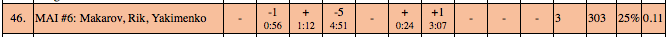
\includegraphics[width=0.95\textwidth]{OC_Ukraine/result.png}\\ [1cm]
\end{center}

\textbf{{\large Ссылка на контест: \url{http://opentrains.snarknews.info/~ejudge/team.cgi?contest_id=10321}}}

\newpage
\textbf{{\large Задача C - Cool Numbers}}

\begin{center}
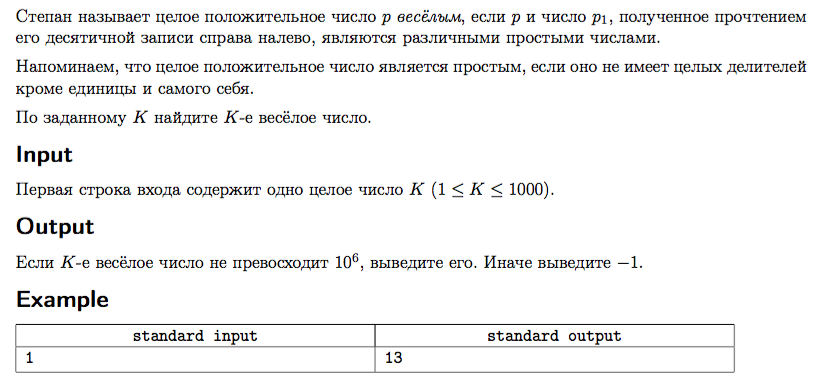
\includegraphics[width=0.9\textwidth]{OC_Ukraine/C.png}\\ [1cm]
\end{center}

\textbf{{\large Алгоритм}}

Для решения данной задачи можно написать генератор весёлых чисел, который посчитает первые 1000 весёлых чисел, а затем уже выводить ответ используя сгенерированные числа. Cложность решения $O(1)$. \\

%\newpage
\textbf{{\large Исходный код}} \\
\begin{lstlisting}[language=C]
#include <iostream>
int main(int argc, const char * argv[]) {
    int nums[] = {13,  17, .. (generated numbers) .., 70529,  70573};
    int k;
    std::cin >> k;
    std::cout << nums[k - 1];
    return 0;
}
\end{lstlisting}


\newpage
\textbf{{\large Задача D - Diagram}}

\begin{center}
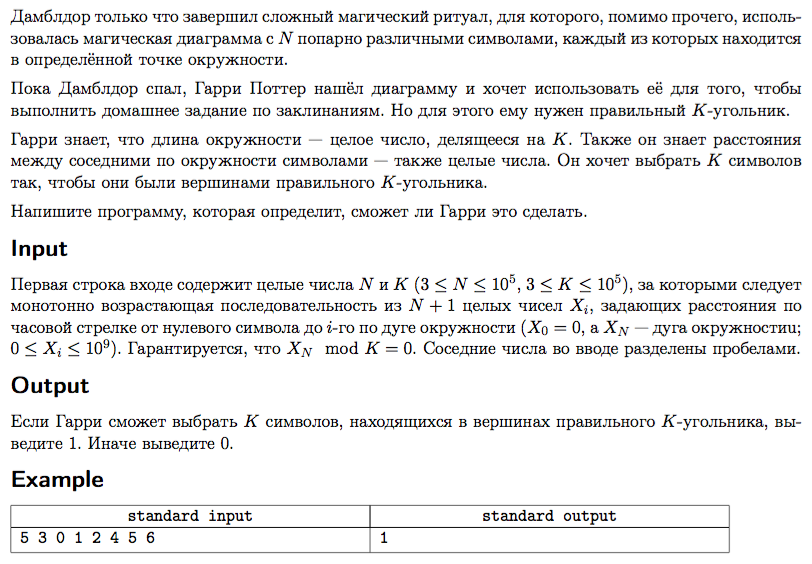
\includegraphics[width=0.9\textwidth]{OC_Ukraine/D.png}\\ [1cm]
\end{center}

\textbf{{\large Алгоритм}}

В этой задаче можно воспользоваться хитростью. Так как нужное количество чисел чтобы построить окружность не поместится в памяти, будем использовать битовый массив, показывающий наличие точки на окружности в заданных координатах. Затем просто пройдем по массиву и попытаемся собрать нужную последовательность. Сложность алгоритма $O(N * K)$.

\newpage
\textbf{{\large Исходный код}} \\
\begin{lstlisting}[language=C]
#include <stdio.h>
#include <stdlib.h>
#include <stdbool.h>
#define ULL unsigned long long
int main() {
    ULL *array = (ULL *)malloc(15500000 * sizeof(ULL));
    ULL p;
    for (p = 0; p < 15000000; p++) {
        array[p] = 0;
    }
    ULL N, K;
    scanf("%lld %lld", &N, &K);
    ULL i;
    int r = 64;
    for (i = 0; i < N; i++) {
        ULL dist;
        scanf("%lld", &dist);
        array[dist/r] |= (1LL << (dist % r));
    }
    ULL max_length;
    scanf("%lld", &max_length);
    const ULL part_size = max_length / K;
    for (i = 0; i < part_size; i++) {
        ULL index = i / r;
        int shift = i % r;
        bool found = true;
        if (array[index] & (1LL << shift)) {
            ULL j;
            for (j = i + part_size; j < max_length; j += part_size) {
                ULL j_index = j / r;
                int j_shift = j % r;
                if (!(array[j_index] & (1LL << j_shift))) {
                    found = false;
                    break;
                }
            }
            if (found) {
                printf("1\n");
                return 0;
            }
        }
    }
    printf("0\n");
    return 0;
}
\end{lstlisting}


\newpage
\textbf{{\large Задача F - First And Last}}

\begin{center}
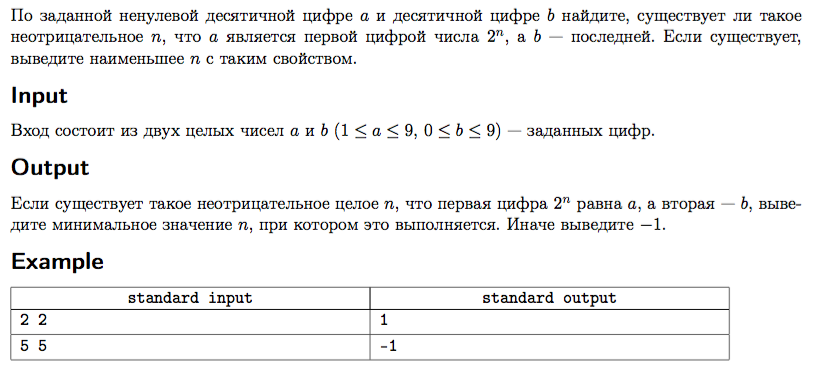
\includegraphics[width=0.9\textwidth]{OC_Ukraine/F.png}\\ [1cm]
\end{center}

\textbf{{\large Алгоритм}}

Задача решается простым перебором. Перебираются все степени двойки до 1000(больше числа быть не может), если попадается подходящие под условие число, то выводим порядок степени и выходим. Если не попадается, то выводим -1. \\


%\newpage
\textbf{{\large Исходный код}} \\
\begin{lstlisting}[language=Perl]
#!/usr/bin/perl
use bigint;
my($a, $b) = split " ", <>;
my $p = 1;
for my $n (0..1000) {
	if (($a eq $b && $p eq $a) || $p =~ m/^$a.*?$b$/) {
		print $n, "\n";
		exit;
	}
	$p <<= 1;
}
print "-1\n";
\end{lstlisting}


\newpage
\textbf{{\large Задача G - Game of Solitaire}}

\begin{center}
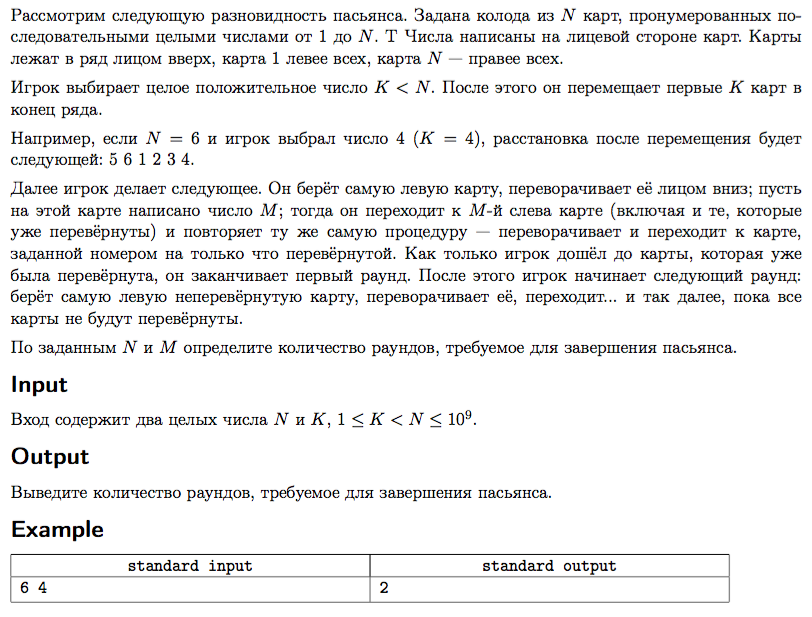
\includegraphics[width=0.9\textwidth]{OC_Ukraine/G.png}\\ [1cm]
\end{center}

\textbf{{\large Алгоритм}}

В этой задаче нужно заметить, что ответом будет наибольший общий делитель входных чисел. НОД находим с помощью алгоритма Евклида. Сложность решения $O(log * min(a, b)$ \\


%\newpage
\textbf{{\large Исходный код}} \\
\begin{lstlisting}[language=C]
#include <iostream>
using namespace std;
long gcd (long a, long b) {
    while (b) {
        a %= b;
        swap(a, b);
    }
    return a;
}
int main() {
    long n, k;
    cin >> n >> k;
    cout << gcd(n, k);
    return 0;
}
\end{lstlisting}






%----------------------------------------------------------------------------------------
%
%	OpenCup GrandPrix of Japan
%
%----------------------------------------------------------------------------------------
\newpage
\subsection{OpenCup GrandPrix of Japan}

\textbf{{\large Результаты}} \\
\begin{center}
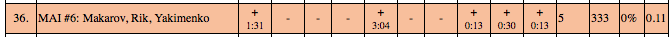
\includegraphics[width=0.95\textwidth]{OC_Japan/result.png}\\ [1cm]
\end{center}

\textbf{{\large Ссылка на контест: \url{http://opentrains.snarknews.info/~ejudge/team.cgi?contest_id=10322}}}


\newpage
\textbf{{\large Задача A - Where is the Boundary}} \\

\begin{center}
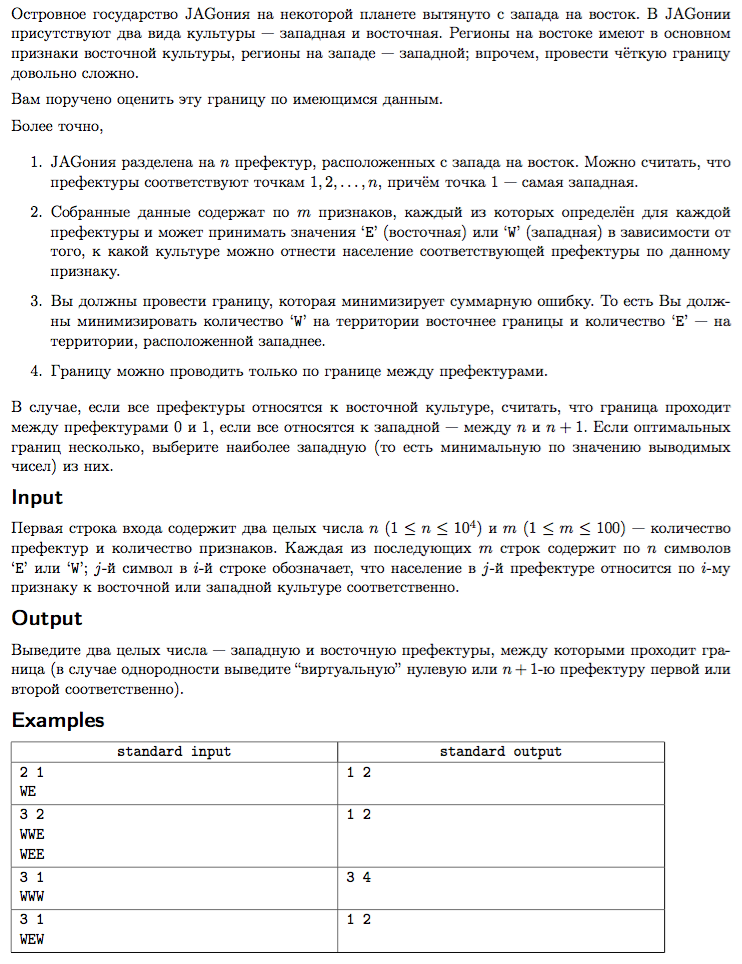
\includegraphics[width=0.9\textwidth]{OC_Japan/A.png}\\ [1cm]
\end{center}

\textbf{{\large Алгоритм}}

В этой задаче нужно просто считать все данные и перебрать все значения ошибок, запоминая индексы минимальных значений. Сложность $O(N * M)$.

\newpage
\textbf{{\large Исходный код}} \\
\begin{lstlisting}[language=C]
#include <iostream>
#include <vector>
#include <map>
using namespace std;
typedef struct {
    int left;
    int rigth;
    int sum;
} error;
int main(int argc, const char * argv[]) {
    int n, m;
    cin >> n >> m;
    vector< map<string,int> > jag(n);
    for (int i = 0; i < n; i++) {
        jag[i]["w"] = 0;
        jag[i]["e"] = 0;
    }
    vector<error> errors (n + 1);
    errors[0].left = 0;
    errors[0].rigth = 0;
    errors[0].sum = 0;
    for (int i = 0; i < m; i++) {
        string features;
        cin >> features;
        for (size_t j = 0; j < features.size(); j++) {
            if (features[j] == 'W') {
                jag[j]["w"]++;
                errors[0].rigth++; // !!!!!!
            } else {
                jag[j]["e"]++;
            }
        }
    }
    errors[0].sum = errors[0].left + errors[0].rigth;
    int min_error = errors[0].rigth;
    int min_error_index = -1;
    for (int i = 1; i < n + 1; i++) {
        errors[i].left = 0;
        errors[i].rigth = 0;
        errors[i].sum = 0;
        errors[i].left = errors[i - 1].left + jag[i - 1]["e"];
        errors[i].rigth = errors[i - 1].rigth - jag[i - 1]["w"];
        errors[i].sum = errors[i].left + errors[i].rigth;   
        if (errors[i].sum < min_error) {
            min_error = errors[i].sum;
            min_error_index = i;
        }
    }
    if (min_error_index == -1) {
        cout << "0 1" << endl;
    } else {
        cout << min_error_index << " " << min_error_index + 1 << endl;
    }   
    return 0;
}
\end{lstlisting}


\newpage
\textbf{{\large Задача G - Surface Area of Cubes}} \\

\begin{center}
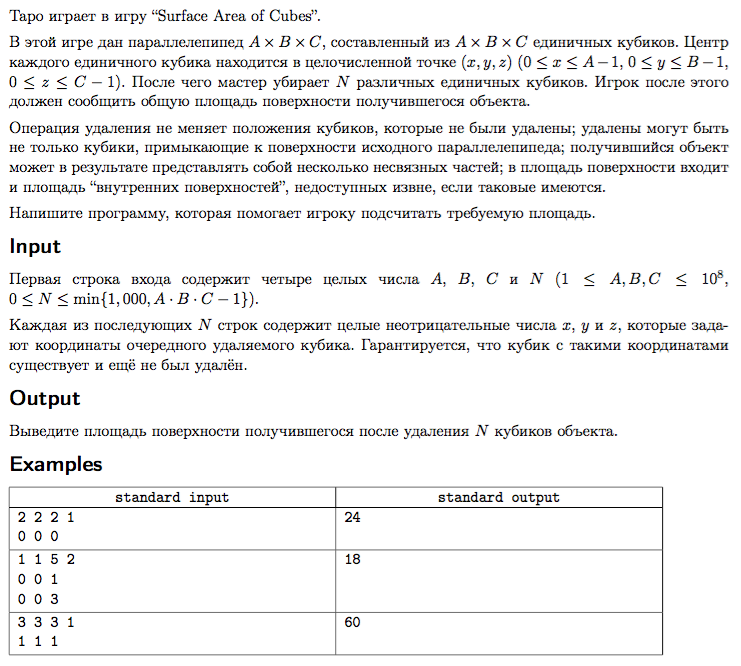
\includegraphics[width=0.9\textwidth]{OC_Japan/G.png}\\ [1cm]
\end{center}

\textbf{{\large Алгоритм}}

Данная задача на реализацию. Необходимо грамотно выстроить структуру и уметь находить изменение площади кубика после убирания кубика на заданных координатах. Сложность $O(N^2)$.

\newpage
\textbf{{\large Исходный код}} \\
\begin{lstlisting}[language=C]
#include <iostream>
#include <vector>
using namespace std;
#define ll long long
class Point {
public:
	ll x, y, z;
	Point() {}
	Point(ll a, ll b, ll c) {
		x = a;
		y = b;
		z = c;
	}
	void setPoints(ll a, ll b, ll c) {
		x = a;
		y = b;
		z = c;
	}
	bool eql(ll a, ll b, ll c) {
		return a == x && b == y && c == z;
	}
};
int main() {
	ll a, b, c, n;
	cin >> a >> b >> c >> n;
	vector<Point> points(n);
	ll square = 2*(a*b + b*c + a*c);
	for (int i = 0; i < n; ++i) {
		ll x, y, z;
		cin >> x >> y >> z;
		points[i].setPoints(x, y, z);
		ll s = 0;
		if (x == 0) ++s;
		if (x == a-1) ++s;
		if (y == 0) ++s;
		if (y == b-1) ++s;
		if (z == 0) ++s;
		if (z == c-1) ++s;
		ll p = 0;
		for (int j = 0; j < i; ++j) {
			if (points[j].eql(x-1, y, z)) ++p;
			if (points[j].eql(x+1, y, z)) ++p;
			if (points[j].eql(x, y-1, z)) ++p;
			if (points[j].eql(x, y+1, z)) ++p;
			if (points[j].eql(x, y, z-1)) ++p;
			if (points[j].eql(x, y, z+1)) ++p;
		}
		square += 6-2*(s+p);
	}
	cout << square << "\n";
	return 0;
}
\end{lstlisting}



\newpage
\textbf{{\large Задача K - Emoticon Counter}} \\

\begin{center}
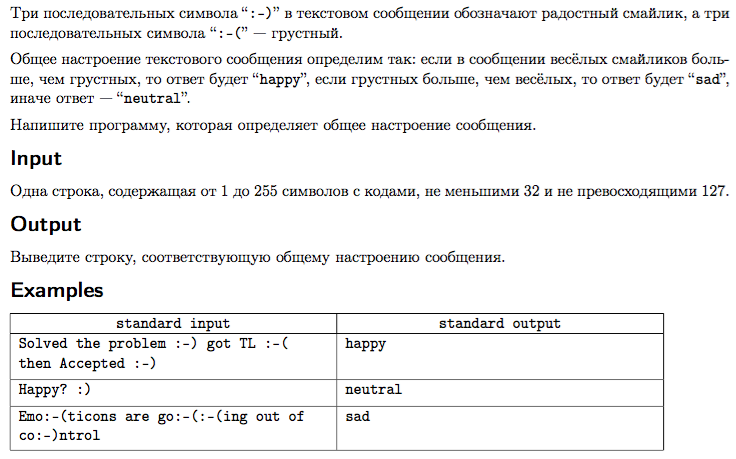
\includegraphics[width=0.9\textwidth]{OC_Japan/K.png}\\ [1cm]
\end{center}

\textbf{{\large Алгоритм}}

В этой задаче необходимо найти все вхождения радостных и грустный смайликов и вывести в ответе каких больше. Решается поиском подстроки в строке. Сложность $O(N * M)$. \\

%\newpage
\textbf{{\large Исходный код}} \\
\begin{lstlisting}[language=Ruby]
str = gets
str = str + "$"
happy = str.split(":-)")
sad = str.split(":-(")
if happy.size > sad.size
  puts "happy"
elsif happy.size < sad.size
  puts "sad"
else
  puts "neutral"
end
\end{lstlisting}


\newpage
\textbf{{\large Задача L - Rogue Language}} \\

\begin{center}
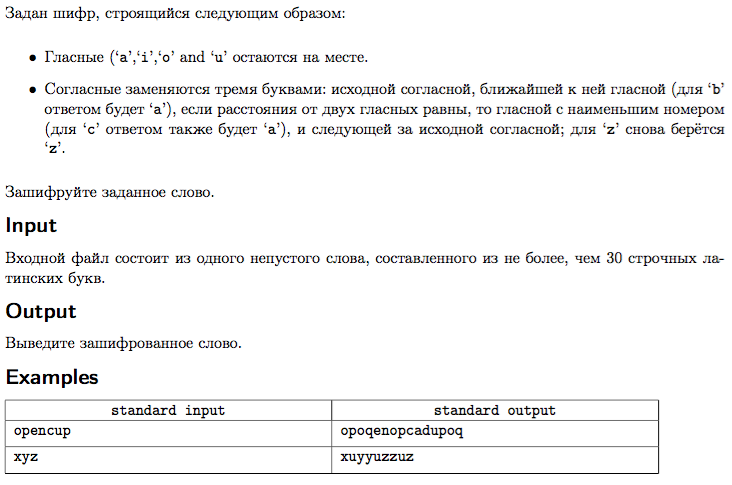
\includegraphics[width=0.9\textwidth]{OC_Japan/L.png}\\ [1cm]
\end{center}

\textbf{{\large Алгоритм}}

В этой задаче нужно понять как меняются символы и просто сделать замену всех символов по составленному словарю замен. Сложность $O(1)$. \\

%\newpage
\textbf{{\large Исходный код}} \\
\begin{lstlisting}[language=Perl]
#!/usr/bin/perl
my %h = (
		a => "a", b => "bac",c => "cad",e => "e",f => "feg",
		g => "geh",h => "hij",i => "i",j => "jik",k => "kil",
		l => "lim",m => "mon",n => "nop",o => "o",p => "poq",
		q => "qor",r => "ros",s => "sut",t => "tuv",u => "u",
		v => "vuw",w => "wux",x => "xuy",y => "yuz",z => "zuz");
my $a = <>;
chomp $a;
my $res = "";
for my $i (split "", $a) {
	$res .= $h{$i};
}
print $res, "\n";
\end{lstlisting}


\newpage
\textbf{{\large Задача M - RPS}} \\

\begin{center}
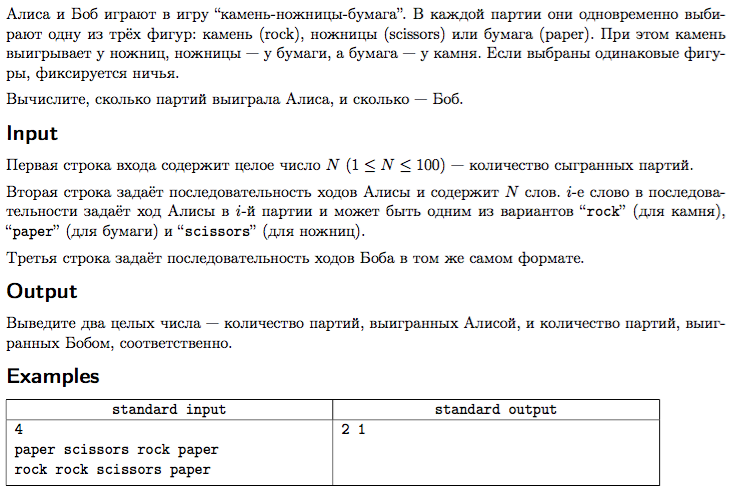
\includegraphics[width=0.9\textwidth]{OC_Japan/M.png}\\ [1cm]
\end{center}

\textbf{{\large Алгоритм}}

В этой задаче упор на реализацию. Нужно просто пройти по входным строкам и сосчитать количество выигрышных партий у каждого из игроков. Сложность $O(N)$.

\newpage
\textbf{{\large Исходный код}} \\
\begin{lstlisting}[language=Perl]
#!/usr/bin/perl
my %h = (paper => 0, scissors => 1, rock => 2);
my $n = <>;
my $A = <>;
my $B = <>;
chomp $A;
chomp $B;
my @A = split " ", $A;
my @B = split " ", $B;
my ($ac, $bc) = (0, 0);
for (my $i = 0; $i < $n; ++$i) {
	my ($a, $b) = ($A[$i], $B[$i]);
	if ($a eq "paper" && $b eq "rock") {
		++$ac;
	}
	elsif ($b eq "paper" && $a eq "rock") {
		++$bc;
	}
	elsif ($h{$a} > $h{$b}) {
		++$ac;
	}
	elsif ($h{$a} < $h{$b}) {
		++$bc;
	}
}
print "$ac $bc\n";
\end{lstlisting}



%----------------------------------------------------------------------------------------
%
%	OpenCup GrandPrix of Eurasia
%
%----------------------------------------------------------------------------------------

\newpage
\subsection{OpenCup GrandPrix of Eurasia)}

\textbf{{\large Результаты}} \\
\begin{center}
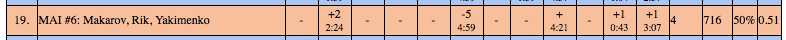
\includegraphics[width=0.95\textwidth]{OC_Eurasia/result.png}\\ [1cm]
\end{center}

\textbf{{\large Ссылка на контест: \url{http://opentrains.snarknews.info/~ejudge/team.cgi?contest_id=10323}}}

\newpage
\textbf{{\large Задача 2 - Плэй-офф}}

\begin{center}
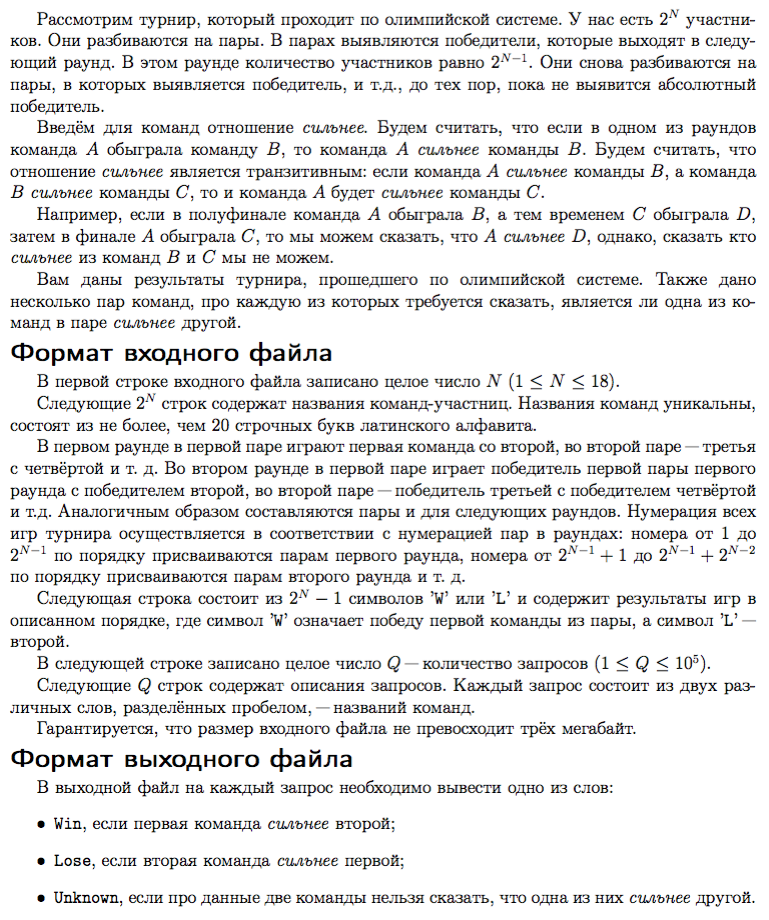
\includegraphics[width=0.9\textwidth]{OC_Eurasia/2_1.png}\\ [1cm]
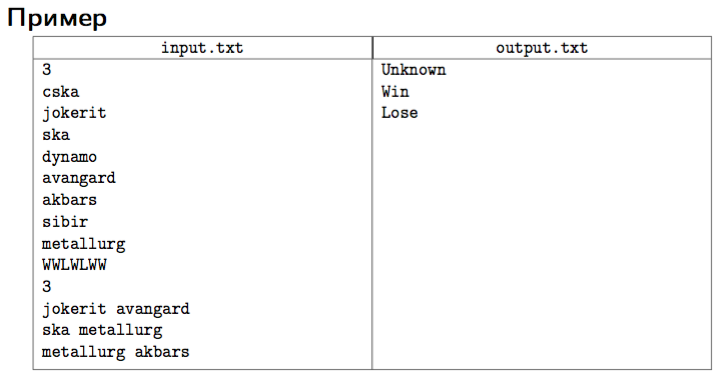
\includegraphics[width=0.6\textwidth]{OC_Eurasia/2_2.png}\\ [1cm]
\end{center}

\textbf{{\large Алгоритм}}

Задача на реализацию. Мы строим дерево команд и каждой команде ставим в соответствие массив команд, которые слабее рассматриваемой. Затем мы считываем запросы и выводим ответ. Сложность алгоритма $O(Q * N * log(N))$.

\newpage
\textbf{{\large Исходный код}} \\
\begin{lstlisting}[language=C]
#include <iostream>
#include <vector>
#include <map>
#include <algorithm>
#include <fstream>
using namespace std;
typedef struct {
    string name;
    vector<string> losers;
} Team;
int main(int argc, const char * argv[]) {
    ifstream in("input.txt");
    ofstream out("output.txt");
    int n;
    in >> n;
    int t = 1;
    for (int i = 0; i < n; i++) {
        t *= 2;
    }
    map<int, vector<int> > teams; // first=team_name, second=losers_vector
    map<string, int> index_for_name;
    vector<pair<int, int> > pairs;
    vector<pair<int, int> > prev_pairs;
    vector<char> log(t - 1);
    for (int i = 0; i < t; i = i + 2) {
        string team_name_1, team_name_2;
        in >> team_name_1 >> team_name_2;
        index_for_name[team_name_1] = i;
        index_for_name[team_name_2] = i + 1;
        teams[i] = vector<int> ();
        teams[i + 1] = vector<int> ();
        pairs.push_back(make_pair(i, i + 1));
    }
    in.get();
    for (int i = 0; i < t - 1; i++) {
        char result = in.get();
        log[i] = result;
    }
    in.get();
    prev_pairs = pairs;
    pairs.clear();
    bool end = false;
    while (!end) {
        for (int i = 0; i < t / 2; i += 2) {
            int first_winner, first_looser;
            int second_winner, second_looser;
            if (log[i] == 'W') {
                first_winner = prev_pairs[i].first;
                first_looser = prev_pairs[i].second;
                teams[first_winner].push_back(first_looser);
                teams[first_winner].insert(teams[first_winner].end(), teams[first_looser].begin(), teams[first_looser].end());
            } else {
                first_winner = prev_pairs[i].second;
                first_looser = prev_pairs[i].first;
                teams[first_winner].push_back(first_looser);
                teams[first_winner].insert(teams[first_winner].end(), teams[first_looser].begin(), teams[first_looser].end());
            }
            if (i == t - 2) {
                end = true;
                break;
            }
            if (log[i + 1] == 'W') {
                second_winner = prev_pairs[i + 1].first;
                second_looser = prev_pairs[i + 1].second;
                teams[second_winner].push_back(second_looser);
                teams[second_winner].insert(teams[second_winner].end(), teams[second_looser].begin(), teams[second_looser].end());
            } else {
                second_winner = prev_pairs[i + 1].second;
                second_looser = prev_pairs[i + 1].first;
                teams[second_winner].push_back(second_looser);
                teams[second_winner].insert(teams[second_winner].end(), teams[second_looser].begin(), teams[second_looser].end());
            }
            pairs.push_back(make_pair(first_winner, second_winner));
        }
        log.erase(log.begin(), log.begin() + t / 2);
        prev_pairs = pairs;
        pairs.clear();
        t /= 2;
    }
    int q;
    in >> q;
    for (int i = 0; i < q; i++) {
        string t1, t2;
        in >> t1 >> t2;
        int index_1 = index_for_name[t1];
        int index_2 = index_for_name[t2];
        if (find(teams[index_1].begin(), teams[index_1].end(), index_2) != teams[index_1].end()) {
            out << "Win" << endl;
        } else if (find(teams[index_2].begin(), teams[index_2].end(), index_1) != teams[index_2].end()) {
            out << "Lose" << endl;
        } else {
            out << "Unknown" << endl;
        }
    }
    in.close();
    out.clear();
    return 0;
}
\end{lstlisting}


\newpage
\textbf{{\large Задача 9 - Хэш-функция}}

\begin{center}
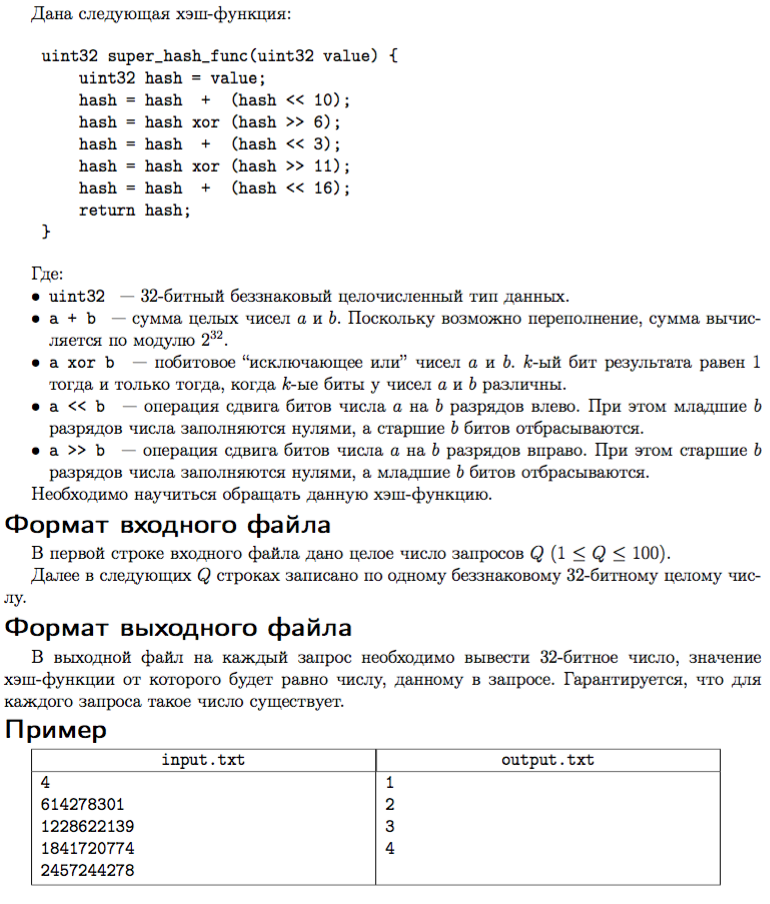
\includegraphics[width=0.9\textwidth]{OC_Eurasia/9.png}\\ [1cm]
\end{center}

\textbf{{\large Алгоритм}}

В каждой операции можно заметить некоторую закономерность, по которой можно получить обратную операцию с использованием некоторого перебора. Обратив таким образом все операции, можно получить искомое число. \\

\newpage
\textbf{{\large Исходный код}} \\
\begin{lstlisting}[language=C]
#include <iostream>
#include <cinttypes>
using namespace std;
#define ll long long
#define ull unsigned long long

uint32_t dehash(uint32_t value) {
    uint32_t hash = value;
    hash = hash - (hash<<16);
    uint32_t t = hash;
	hash = (hash xor (hash >> 11)) & ~((1ULL<<10)-1);
	for (int i = 0; i < 1023; ++i) {
		if ((hash xor (hash >> 11)) == t) {
			break;
		}
		++hash;
	}
	ull h = hash;
	for (ull i = 0;; ++i) {
		if (((h|(i<<32)) % 9) == 0) {
			hash = (h|(i<<32))/9;
			break;
		}
	}
	t = hash;
	hash = (hash xor (hash >> 6)) & ~((1ULL<<20)-1);
	for (int i = 0; i < 1048575; ++i) {
		if ((hash xor (hash >> 6)) == t) {
			break;
		}
		++hash;
	}
	h = hash;
	for (ull i = 0;; ++i) {
		if (((h|(i<<32)) % 1025) == 0) {
			hash = (h|(i<<32))/1025;
			break;
		}
	}
    return hash;
}

int main() {
	uint32_t Q;
	cin >> Q;
	for (int i = 0; i < Q; ++i) {
		ull d;
		cin >> d;
		cout << dehash(d) << "\n";
	}
	return 0;
}
\end{lstlisting}


\newpage
\textbf{{\large Задача 11 - Стулья мастера Гамбса}}

\begin{center}
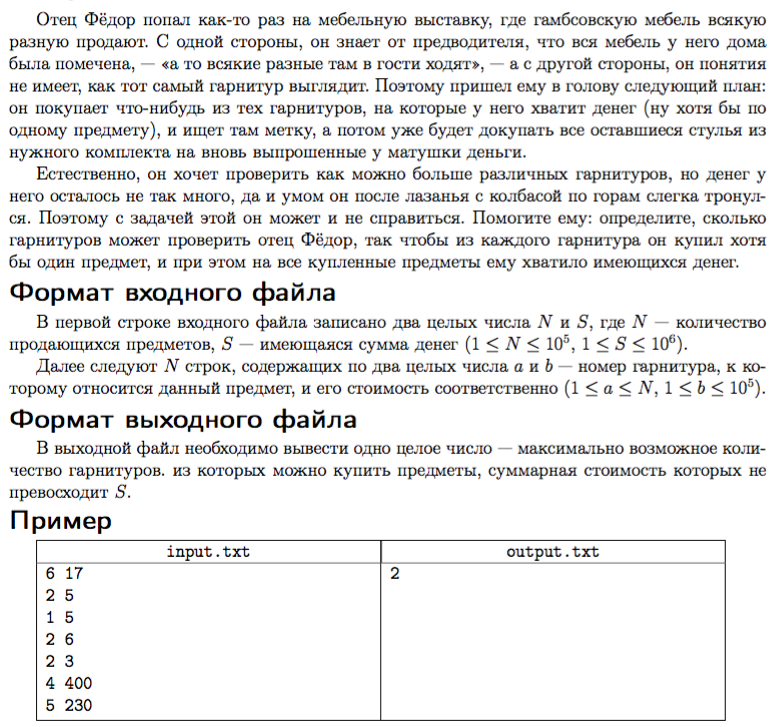
\includegraphics[width=0.9\textwidth]{OC_Eurasia/11.png}\\ [1cm]
\end{center}

\textbf{{\large Алгоритм}}

Для решения данной задачи мы отсортируем стулья по стоимости, а затем будем набирать стулья начиная с самых дешевых. Если находим стул, который не можем купить, то завершаем выполнение, так как дальше не будет стульев которые мы сможем купить. Сложность алгоритма $O(N^2 * log(N)$.

\newpage
\textbf{{\large Исходный код}} \\
\begin{lstlisting}[language=C]
#include <iostream>
#include <algorithm>
#include <fstream>
#include <vector>

using namespace std;

bool pairMinMax(const pair<int, int> &a, const pair<int, int> &b) {
	return a.second < b.second;
}


int main() {

	ifstream in("input.txt");
	ofstream out("output.txt");


	int N;
	long long S;

	in >> N >> S;

	vector <pair <int, int> > element(N);
	vector <bool> bought(N+1, false);

	pair <int, int> temp;
	for (int i = 0; i < N; i++) {
		in >> temp.first >> temp.second;
		element[i] = temp;
	}

	sort(element.begin(), element.end(), pairMinMax);

	int count = 0;
	for (int i = 0; i < N; i++) {
		if (element[i].second > S) {
			break;
		}
		if (element[i].second <= S && bought[element[i].first] == false) {
			S -= element[i].second;
			bought[element[i].first] = true;
			count++;
		}
	}

	out << count << endl;
	
	in.close();
	out.close();

	return 0;
}
\end{lstlisting}


\newpage
\textbf{{\large Задача 12 - Эрудит}}

\begin{center}
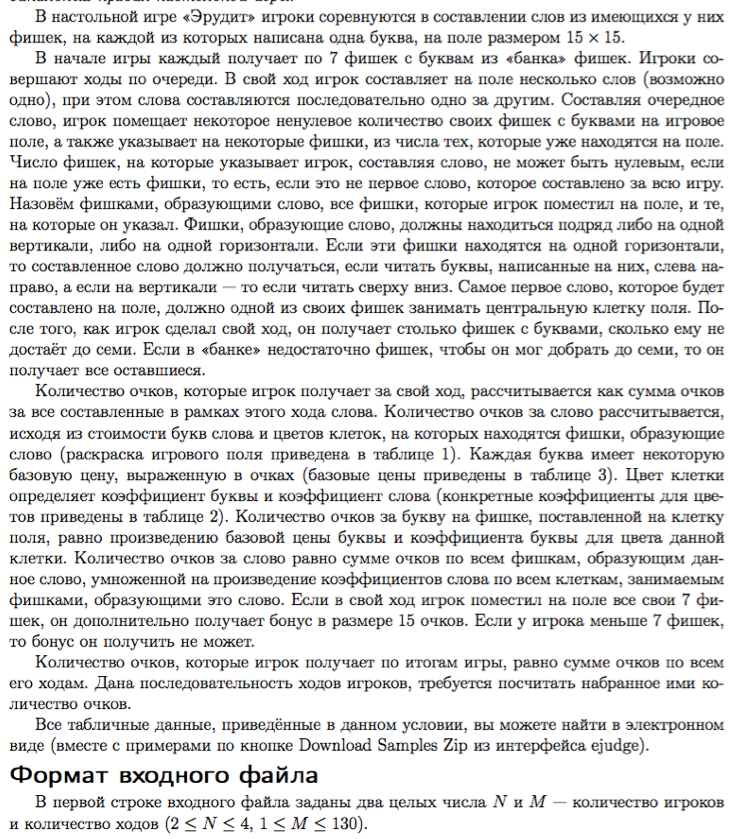
\includegraphics[width=0.9\textwidth]{OC_Eurasia/12_1.png}\\ [1cm]
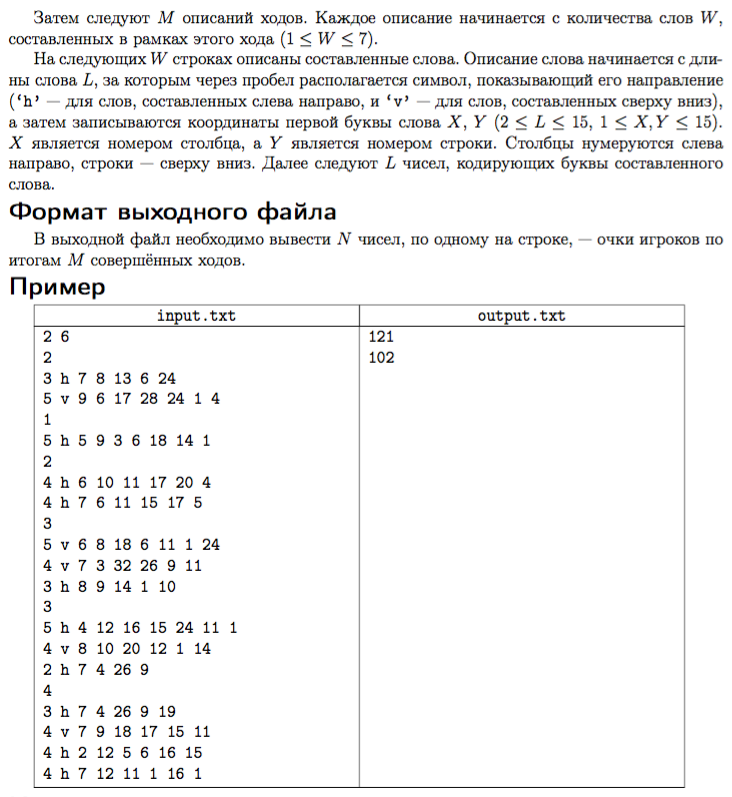
\includegraphics[width=0.9\textwidth]{OC_Eurasia/12_2.png}\\ [1cm]
\end{center}

\textbf{{\large Алгоритм}}

Эта задача на реализацию. Требуется просто запрограммировать все действия, описанные в условии. \\

\newpage
\textbf{{\large Исходный код}} \\
\begin{lstlisting}[language=Perl]
#!/usr/bin/perl
use bigint;
my @cmap = qw(  rwwgwwwrwwwgwwr
				wbwwwywwwywwwbw
				wwbwwwgwgwwwbww
				gwwbwwwgwwwbwwg
				wwwwbwwwwwbwwww
				wywwwwwwwwwwwyw
				wwgwwwgwgwwwgww
				rwwgwwwswwwgwwr
				wwgwwwgwgwwwgww
				wywwwwwwwwwwwyw
				wwwwbwwwwwbwwww
				gwwbwwwgwwwbwwg
				wwbwwwgwgwwwbww
				wbwwwywwwywwwbw
				rwwgwwwrwwwgwwr);
my @map;
for (my $i = 0; $i < 16; ++$i) {
	for (my $j = 0; $j < 16; ++$j) {
		$map[$i][$j] = 0;
	}
}
my @alp = (1,3,2,3,2,1,5,5,1,2,2,2,2,1,1,2,2,2,2,3,10,5,10,5,10,10,10,5,5,10,10,3);

my %cl = 
   (w => 1,
    s => 1,
    g => 2,
    y => 3,
    b => 1,
    r => 1);

my %cw = 
   (w => 1,
    s => 1,
    g => 1,
    y => 1,
    b => 2,
    r => 3);

sub getColor {
	my ($x, $y) = @_;
	substr $cmap[$y-1], $x-1, 1;
}
my $str;
$str = <ARGV>;
chomp $str;
my ($n, $m) = split(" ", $str);
my @scores;
for (my $i = 0; $i < $n; ++$i) {
	$scores[$i] = 0;
}
for (my $si = 0; $si < $m; ++$si) {
	my $str = <ARGV>;
	chomp $str;
	my $w = $str;
	my $count = 0;
	my $score = 0;
	for (my $i = 0; $i < $w; ++$i) {
		$str = <ARGV>;
		chomp $str;
		my @A = split(" ", $str);
		my $l = shift @A;
		my $dir = shift @A;
		my $x = shift @A;
		my $y = shift @A;
		my $scoreL = 0;
		my $scoreW = 1;
		for my $char (@A) {
			my $color = getColor($x, $y);
			unless ($map[$x][$y]) {
				$map[$x][$y] = 1;
				++$count;
			}

			$scoreL += $cl{$color} * $alp[$char-1];
			$scoreW *= $cw{$color};
			if ($dir eq 'v') {
				++$y;
			}
			else {
				++$x;
			}
		}
		$score += $scoreW * $scoreL;
	}
	if ($count == 7) {
		$score += 15;
	}
	$scores[$si%$n] += $score;
}
print join("\n", @scores), "\n";
\end{lstlisting}





%----------------------------------------------------------------------------------------
%
%	OpenCup GrandPrix of SPb
%
%----------------------------------------------------------------------------------------

\newpage
\subsection{OpenCup GrandPrix of SPb}

\textbf{{\large Результаты}} \\
\begin{center}
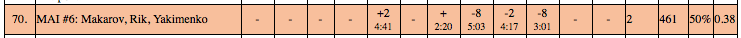
\includegraphics[width=0.95\textwidth]{OC_SPB/result.png}\\ [1cm]
\end{center}

\textbf{{\large Ссылка на контест: \url{http://opentrains.snarknews.info/~ejudge/team.cgi?contest_id=10324}}}

\newpage
\textbf{{\large Задача E - Следующее разбиение}}

\begin{center}
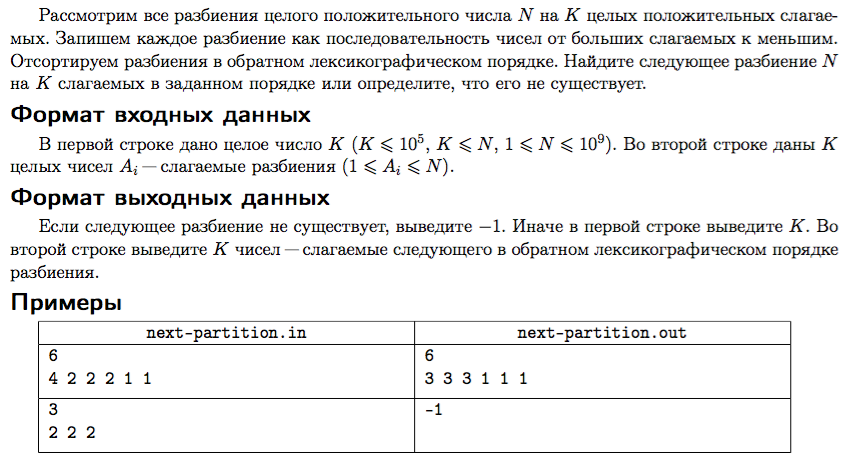
\includegraphics[width=0.9\textwidth]{OC_SPB/E.png}\\ [1cm]
\end{center}

\textbf{{\large Алгоритм}}

Задача решается с помощью перебора с некоторыми оптимизациями. Сложность $O(n^3)$. \\

\textbf{{\large Исходный код}} \\
\begin{lstlisting}[language=C]
#include <iostream>
using namespace std;
bool pairMinMax(const pair<int, int> &a, const pair<int, int> &b) {
	return a.second < b.second;
}
int main() {
	int input;
	ifstream in("next-partition.in");
	ofstream out("next-partition.out");
	int K;
	in >> K;
	vector <int> A(K);
	int N = 0;
	int temp;
	for (int i = 0; i < K; i++) {
		in >> temp;
		A[i] = temp;
		N += temp;
	}
	bool flag1 = false;
	bool flag2 = false;
	int sum = 0;
	sort(A.begin(), A.end());
	int iMarked = 0;
	for (int i = 0; i < K - 1; i++) {
		sum += A[i];
		if (A[i + 1] - A[i] >= 2) {
			iMarked = i + 1;
			A[i + 1]--;
			sum++;
			flag1 = true;
			break;
		}
	}
	if (!flag1) {
		for (int i = 0; i < K - 2; i++) {
			for (int j = i + 2; j < K; j++) {
				if (A[i] + 1 > A[i + 1]) {
					break;
				}
				if (A[j] - A[i] > 2) {
					break;
				}
				if (A[j] - A[i] == 2 && A[j] - 1 >= A[j - 1]) {
					A[j]--;
					A[i]++;
					flag2 = true;
					break;
				}
			}
		}
	}
	if (flag1) {
		sum -= iMarked;
		for (int i = iMarked - 1; i >= 0; i--) {
			if (sum > 0) {
				temp = A[iMarked];
				if (sum+1 >= temp) {
					A[i] = temp;
					sum = sum - temp + 1;
				}
				else {
					A[i] = sum + 1;
					sum = 0;
				}
			}
			else A[i] = 1;
		}
		out << K << endl;
		for (int i = K - 1; i >= 0; i--) {
			out << A[i] << " ";
		}
	}
	else if (flag2) {
		out << K << endl;
		for (int i = K - 1; i >= 0; i--) {
			out << A[i] << " ";
		}
	} else {
		out << -1;
	}
	in.close();
	out.close();
	return 0;
}
\end{lstlisting}


\newpage
\textbf{{\large Задача G - Головоломка Обмен}}

\begin{center}
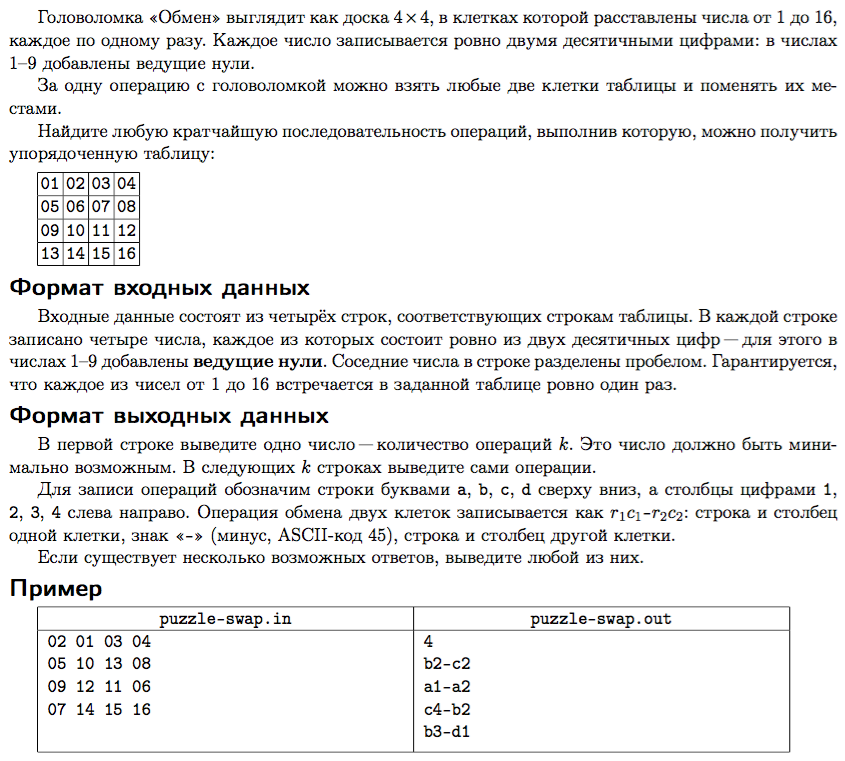
\includegraphics[width=0.9\textwidth]{OC_SPB/G.png}\\ [1cm]
\end{center}

\textbf{{\large Алгоритм}}

Так как доска всегда имеет размеры 4х4, то задачу можно решить полным перебором. Сначала перебором находим все неправильные пары чисел, а затем начинаем исправлять пары переставляя строки, пока доска не станет правильной.

\newpage
\textbf{{\large Исходный код}} \\
\begin{lstlisting}[language=C]
#include <iostream>
#include <sstream>
#include <vector>
#include <fstream>

using namespace std;

bool desk_is_correct(int desk[4][4])
{
    for (int i = 0; i < 4; i++) {
        for (int j = 0; j < 4; j++) {
            int targer_i = (desk[i][j] - 1) / 4;
            int targer_j = (desk[i][j] - 1) % 4;
            if (i != targer_i || j != targer_j) {
                return false;
            }
        }
    }
    return true;
}

char character_for_num(int num)
{
    return char('a' + num);
}

int main(int argc, const char * argv[])
{
    stringstream ss;
    
    ifstream in("puzzle-swap.in");
    ofstream out("puzzle-swap.out");
    
    int desk[4][4] = {0};
    
    for (int i = 0; i < 4; i++) {
        for (int j = 0; j < 4; j++) {
            in >> desk[i][j];
        }
    }
    
    int moves = 0;
    vector<string> log;
    
    // find all wrong pairs
    for (int i1 = 0; i1 < 4; i1++) {
        for (int j1 = 0; j1 < 4; j1++) {
            for (int i2 = 0; i2 < 4; i2++) {
                for (int j2 = 0; j2 < 4; j2++) {
                    if (i1 != i2 || j1 != j2) {
                        int targer_i1 = (desk[i1][j1] - 1) / 4;
                        int targer_j1 = (desk[i1][j1] - 1) % 4;
                        int targer_i2 = (desk[i2][j2] - 1) / 4;
                        int targer_j2 = (desk[i2][j2] - 1) % 4;
                        if (targer_i1 == i2 && targer_j1 == j2 &&
                            targer_i2 == i1 && targer_j2 == j1) {
                            moves++;
                            swap(desk[i1][j1], desk[i2][j2]);
                            ss << character_for_num(i1) << j1 + 1 << "-" << character_for_num(i2) << j2 + 1 << endl;
                            string s;
                            ss >> s;
                            log.push_back(s);
                        }
                    }
                }
            }
        }
    }
    
    while (!desk_is_correct(desk)) {
        for (int i = 0; i < 4; i++) {
            for (int j = 0; j < 4; j++) {
                int targer_i = (desk[i][j] - 1) / 4;
                int targer_j = (desk[i][j] - 1) % 4;
                if (i != targer_i || j != targer_j) {
                    moves++;
                    swap(desk[i][j], desk[targer_i][targer_j]);
                    ss << character_for_num(i) << j + 1 << "-" << character_for_num(targer_i) << targer_j + 1 << endl;
                    string s;
                    ss >> s;
                    log.push_back(s);
                }
            }
        }
    }
    
    out << moves << endl;
    for (size_t i = 0; i < log.size(); i++) {
        out << log[i] << endl;
    }
    
    in.close();
    out.close();
    
    return 0;
}

\end{lstlisting}





%----------------------------------------------------------------------------------------
%
%	ACM 1/4 Final
%
%----------------------------------------------------------------------------------------
\newpage
\subsection{ACM-ICPC Московский четвертьфинал}

Так как соревнование проводилось в ВШЭ, то турнирная таблица с результатами и исходные коды программ не доступны. \\




%----------------------------------------------------------------------------------------
%
%	OpenCup GrandPrix of Yekaterinburg
%
%----------------------------------------------------------------------------------------
\newpage
\subsection{OpenCup GrandPrix of Yekaterinburg}

\textbf{{\large Результаты}} \\
\begin{center}
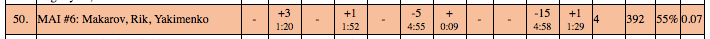
\includegraphics[width=0.95\textwidth]{OC_YKB/result.png}\\ [1cm]
\end{center}

\textbf{{\large Ссылка на контест: \url{http://opentrains.snarknews.info/~ejudge/team.cgi?contest_id=10325}}}

\newpage
\textbf{{\large Задача B - Black Widow}}

\begin{center}
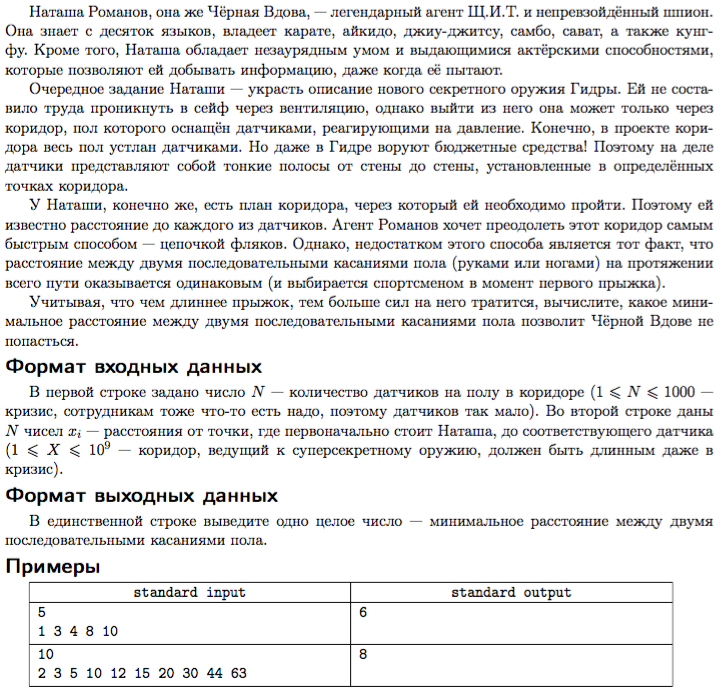
\includegraphics[width=0.9\textwidth]{OC_YKB/B.png}\\ [1cm]
\end{center}

\textbf{{\large Алгоритм}}

Перебираем всевозможные варианты перемещения и выберем тот, у которого расстояние между соседними точками будет минимальным. \\

\newpage
\textbf{{\large Исходный код}} \\
\begin{lstlisting}[language=C]
#include <iostream>
#include <set>
#include <vector>
using namespace std;
#define ll long long
#define ull unsigned long long

int main() {
	ull n;
	cin >> n;
	set<ull> v;
	vector<ull> m;
	ull maxV = 0;
	ull a = 1;
	for (int i = 0; i < n; ++i) {
		ull d;
		cin >> d;
		if (d > maxV)
			maxV = d;
		v.insert(d);
		m.push_back(d);
	}
	bool f = 1;
	while (1) {
		++a;
		bool f = 1;
		for (int i = 0; i < n; ++i) {
			if (m[i] >= a && m[i]%a == 0) {
				f = 0;
				break;
			}
		}
		if (f) {
			break;
		}
	}
	while (1) {
		f = 1;
		for (ull x = 0; x < maxV+1; x += a) {
			if (v.find(x) != v.end()) {
				f = 0;
				break;
			}
		}
		if (f) {
			cout << a << endl;
			break;
		}
		while (1) {
			++a;
			bool f = 1;
			for (int i = 0; i < n; ++i) {
				if (m[i] >= a && m[i]%a == 0) {
					f = 0;
					break;
				}
			}
			if (f) {
				break;
			}
		}
	}
	return 0;
}
\end{lstlisting}


\newpage
\textbf{{\large Задача D - Dr. Banner}}

\begin{center}
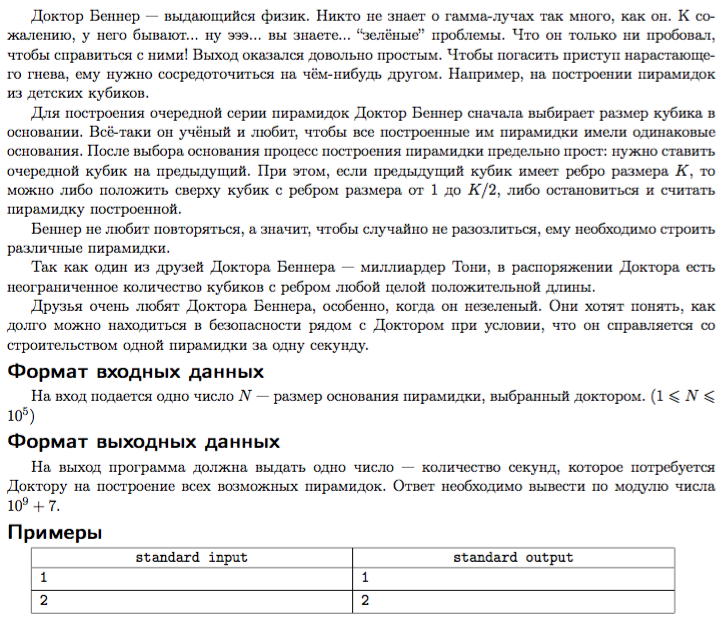
\includegraphics[width=0.9\textwidth]{OC_YKB/D.png}\\ [1cm]
\end{center}

\textbf{{\large Алгоритм}}

Для решения этой задачи нам нужно знать префиксную сумму по времени на отрезке. Мы можем вычислить вручную несколько первых значений, по которым потом сможешь получить любое значение, так как все они высчитываются на основе предыдущих. Сложность алгоритма $O(N)$. \\

\textbf{{\large Исходный код}} \\
\begin{lstlisting}[language=Ruby]
n = gets.to_i
m = (1e+9 + 7).to_i

amount = Array.new(1e+5 + 1)
sum_for_pos = Array.new(1e+5 + 1)

k = 5

amount[1] = 1
amount[2] = 2
amount[3] = 2
amount[4] = 4

sum_for_pos[1] = 1
sum_for_pos[2] = 3
sum_for_pos[3] = 5
sum_for_pos[4] = 9

while k <= n do
    max_next_k = k / 2
    amount[k] = (1 + sum_for_pos[max_next_k])
    sum_for_pos[k] = sum_for_pos[k - 1] + amount[k]
    k += 1
end

answer = (amount[n] % m)

puts answer
\end{lstlisting}



\newpage
\textbf{{\large Задача G - Groot}}

\begin{center}
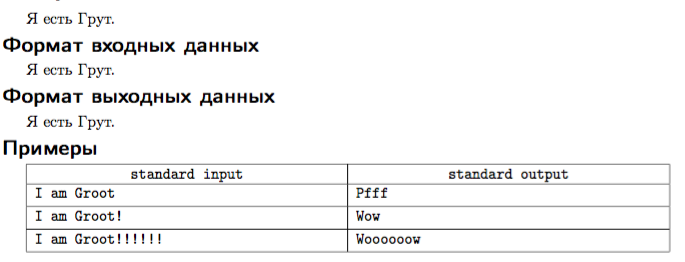
\includegraphics[width=0.9\textwidth]{OC_YKB/G.png}\\ [1cm]
\end{center}

\textbf{{\large Алгоритм}}

В этой задаче нужно посчитать количество восклицательных знаков во входной строке и вывести слово Wow, в котором столько же букв $o$, сколько знаков в строке. Если в строке нет ни одного знака, то вывести Pffff. Сложность $O(1)$. \\

\textbf{{\large Исходный код}} \\
\begin{lstlisting}[language=Perl]
#!/usr/bin/perl
my $str =  <>;
my @a = $str =~ /\!/g;
my $n = scalar(@a);
if ($n == 0) {
	print "Pfff";
}
else {
	print "W"."o"x$n."w";
}
\end{lstlisting}


\newpage
\textbf{{\large Задача L - Loki and Forks}}

\begin{center}
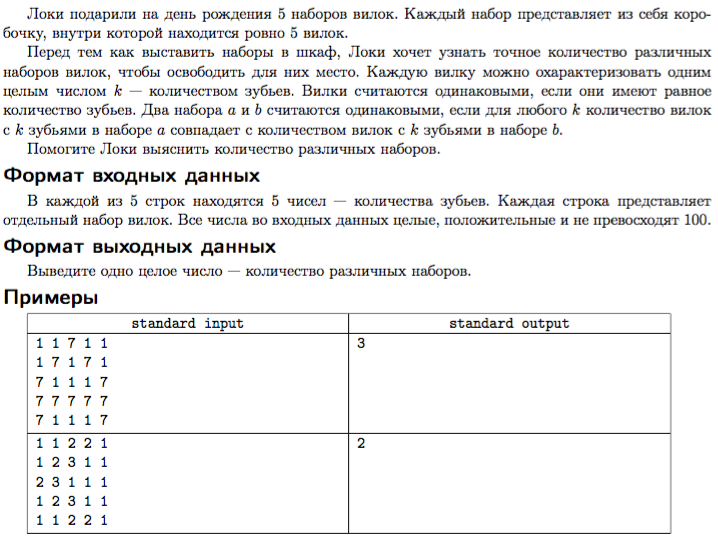
\includegraphics[width=0.9\textwidth]{OC_YKB/L.png}\\ [1cm]
\end{center}

\textbf{{\large Алгоритм}}

Чтобы посчитать количество уникальных наборов нужно просто отсортировать все значения количества зубьев в наборах, затем построить из этих чисел строки путем конкатенирования и посчитать количество уникальных строк. Сложность $O(N * log(N))$. \\

\textbf{{\large Исходный код}} \\
\begin{lstlisting}[language=Perl]
#!/usr/bin/perl
my %h;
while (my $str = <>) {
	chomp $str;
	++$h{join "", sort {$a <=> $b} split " ", $str};
}
print scalar(keys(%h));
\end{lstlisting}







%----------------------------------------------------------------------------------------
%
%	OpenCup GP of Siberia
%
%----------------------------------------------------------------------------------------
\newpage
\subsection{OpenCup GrandPrix of Siberia}

\textbf{{\large Результаты}} \\
\begin{center}
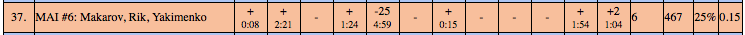
\includegraphics[width=0.95\textwidth]{OC_Siberia/result.png}\\ [1cm]
\end{center}

\textbf{{\large Ссылка на контест: \url{http://opentrains.snarknews.info/~ejudge/team.cgi?contest_id=10281}}}

\newpage
\textbf{{\large Задача А - Detect a Mood}}

\begin{center}
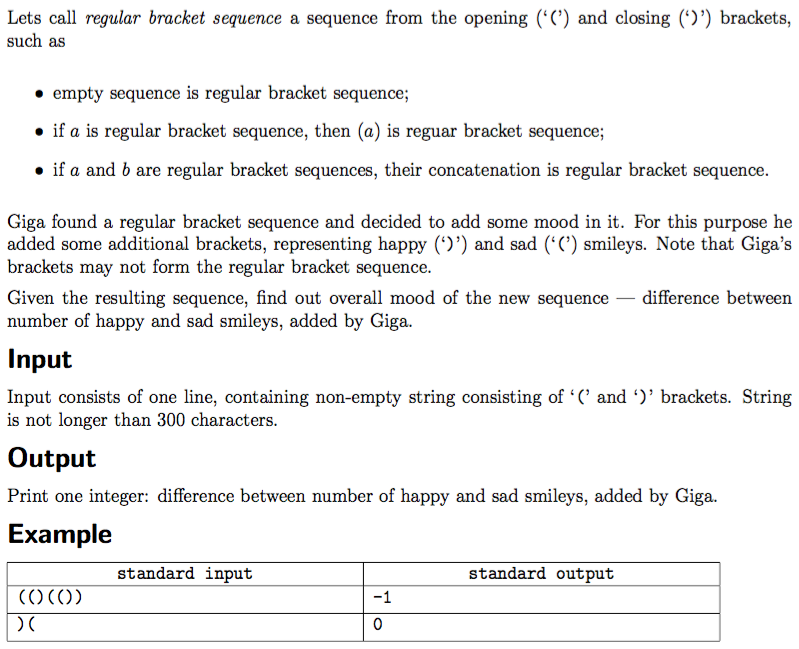
\includegraphics[width=0.9\textwidth]{OC_Siberia/A.png}\\ [1cm]
\end{center}

\textbf{{\large Алгоритм}}

В этой задаче нужно посчитать количество открывающих и закрывающих скобок, а затем найти их разность. Это и будет ответом. Сложность $O(N)$. \\

\textbf{{\large Исходный код}} \\
\begin{lstlisting}[language=Perl]
#!/usr/bin/perl
my $s = <>;
chomp $s;
while ($s =~ s/\(\)//) {}
my $n = length($s);
$s =~ s/\)//g;
my $rn = length($s);
print $n - 2*$rn;
\end{lstlisting}


\newpage
\textbf{{\large Задача B - Painting Tracks}}

\begin{center}
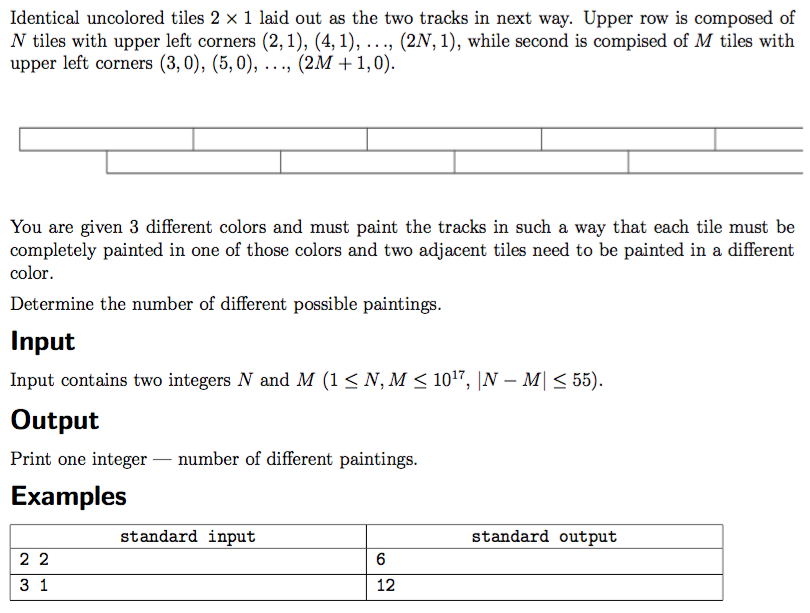
\includegraphics[width=0.9\textwidth]{OC_Siberia/B.png}\\ [1cm]
\end{center}

\textbf{{\large Алгоритм}}

Если $N = M$, то ответ 6. Иначе ответ равен 3 умноженной на 2 в степени разницы между $N$ и $M$. Сложность $O(1)$. \\

\textbf{{\large Исходный код}} \\
\begin{lstlisting}[language=C++]
#include <iostream>
#include <algorithm>
#include <vector>
#include <cmath>
#include <set>

#define LL long long
#define ULL  unsigned long long


using namespace std;

ULL myAbs(ULL a, ULL b) {
	if(a > b) {
		return a - b;
	} else {
		return b - a + 1;
	}
}

int main() {

	int temp;
	ULL N, M;
	cin >> N >> M;
	if(N == M) {
		cout << 6 << endl;
		return 0;
	}
	else {
		ULL answ = 3;
		for(int i = 0; i < myAbs(N, M); i++) {
			answ *= 2;
		}
		cout << answ << endl;
	}

	//cin >> temp;
	
	return 0;

}
\end{lstlisting}


\newpage
\textbf{{\large Задача D - Match of the Giants}}

\begin{center}
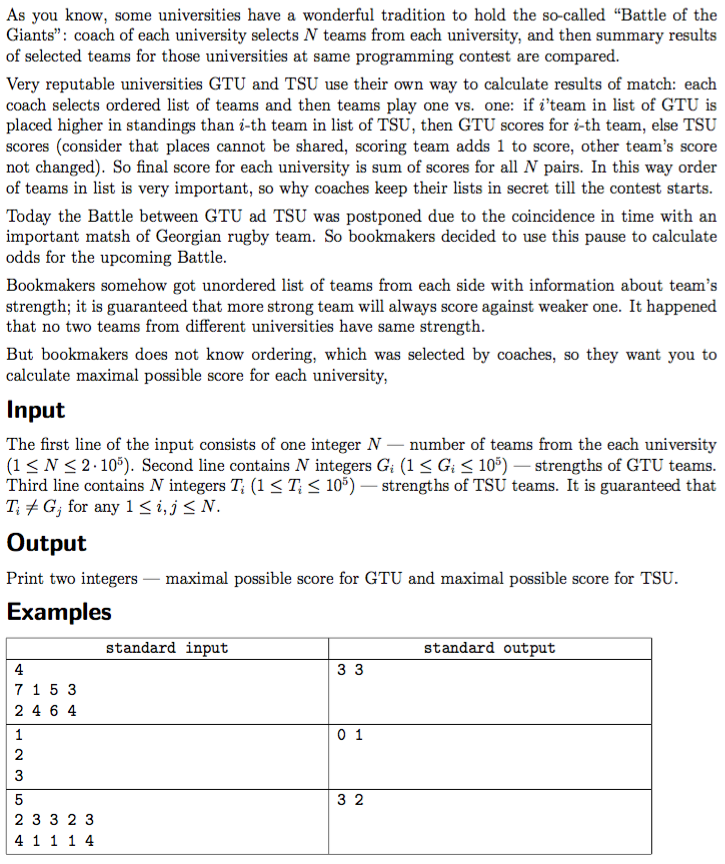
\includegraphics[width=0.9\textwidth]{OC_Siberia/D.png}\\ [1cm]
\end{center}

\textbf{{\large Алгоритм}}

В этой задаче нужно найти максимально возможный счет для каждой команды. Для этого отсортируем значения каждой команды по убыванию и для каждой команды найдем значение в противоположной команде, которое даст максимальный выигрыш. Сложность $O(N * log(N))$. \\

\newpage
\textbf{{\large Исходный код}} \\
\begin{lstlisting}[language=C++]
#include <iostream>
#include <vector>
#include <algorithm>
#include <climits>

using namespace std;

int main(int argc, const char * argv[]) {
    
    int n;
    cin >> n;
    
    vector<int> gtu(n);
    vector<int> tsu(n);
    
    int val;
    
    for (int i = 0; i < n; i++) {
        cin >> val;
        gtu[i] = val;
    }
    
    for (int i = 0; i < n; i++) {
        cin >> val;
        tsu[i] = val;
    }
    
    sort(gtu.begin(), gtu.end(), greater<int>());
    sort(tsu.begin(), tsu.end(), greater<int>());
    
    int gtu_score = 0;
    int tsu_score = 0;
    
    vector<int> tsu_search = tsu;
    
    int next_start_pos = 0;
    
    for (int i = 0; i < n; i++) {
        bool found = false;
        for (int j = next_start_pos; j < n; j++) {
            if (gtu[i] > tsu_search[j]) {
                gtu_score++;
                tsu_search[j] = INT_MAX;
                found = true;
                next_start_pos = j + 1;
                break;
            }
        }
        if (!found) {
            break;
        }
    }
    
    next_start_pos = 0;
    
    for (int i = 0; i < n; i++) {
        bool found = false;
        for (int j = next_start_pos; j < n; j++) {
            if (tsu[i] > gtu[j]) {
                tsu_score++;
                gtu[j] = INT_MAX;
                found = true;
                next_start_pos = j + 1;
                break;
            }
        }
        if (!found) {
            break;
        }
    }
    
    cout << gtu_score << " " << tsu_score << endl;
    
    return 0;
}

\end{lstlisting}


\newpage
\textbf{{\large Задача G - Files list}}

\begin{center}
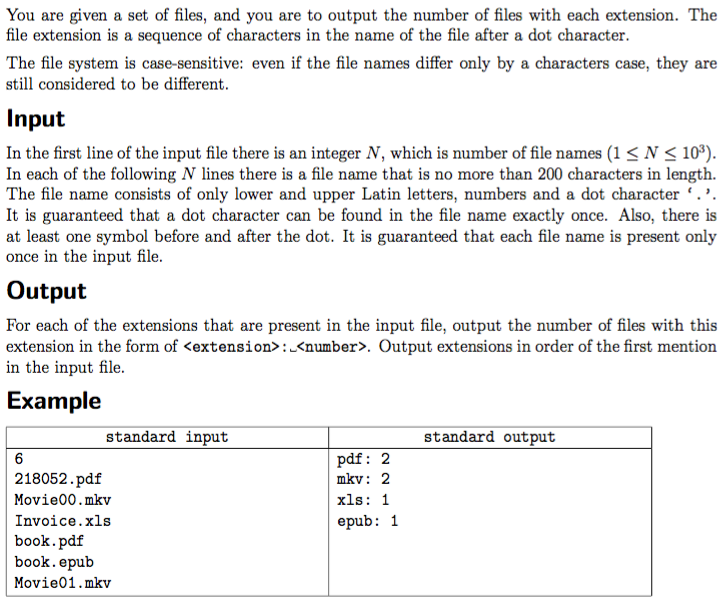
\includegraphics[width=0.9\textwidth]{OC_Siberia/G.png}\\ [1cm]
\end{center}

\textbf{{\large Алгоритм}}

В этой задаче нужно найти количество уникальных расширений файлов. Для этого каждое расширение в строке будем заносить в хеш-таблицу и запоминать количество вхождений. Сложность $O(N * log(N))$. \\

\textbf{{\large Исходный код}} \\
\begin{lstlisting}[language=Perl]
#!/usr/bin/perl
<>;
my %h;
my $i;
my @keys;
while (my $s = <>) {
	chomp $s;
	my ($suf) = $s =~ /\.(.+?)$/;
	push @keys, $suf unless exists $h{$suf};
	++$h{$suf};
}
foreach my $key (@keys) {
	print $key, ": ", $h{$key}, "\n";
}
\end{lstlisting}


\newpage
\textbf{{\large Задача K - Hive}}

\begin{center}
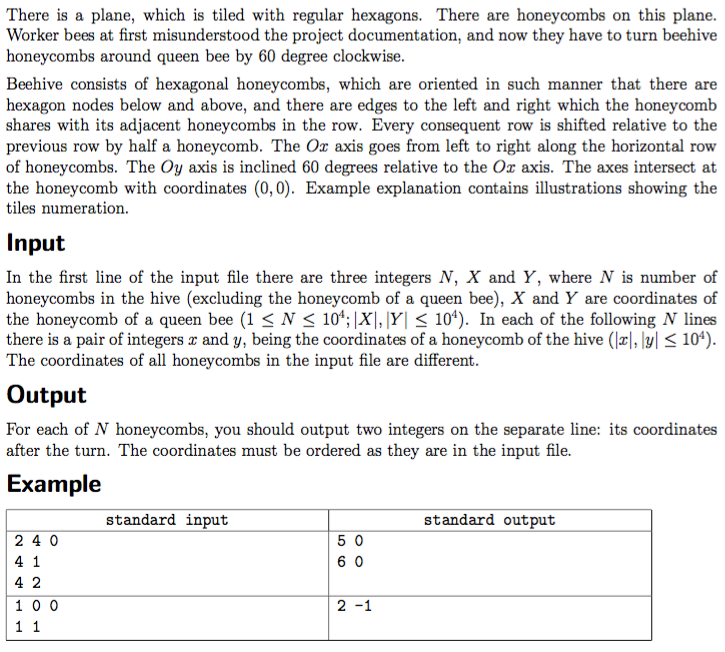
\includegraphics[width=0.9\textwidth]{OC_Siberia/K.png}\\ [1cm]
\end{center}

\textbf{{\large Алгоритм}}

Задача решается с помощью простой формулы, которая находится в исходном коде на 5 строке. Сложность $O(1)$. \\

\textbf{{\large Исходный код}} \\
\begin{lstlisting}[language=Perl]
#!/usr/bin/perl
my ($n, $x0, $y0) = split " ", <>;
for (my $i = 0; $i < $n; ++$i) {
	my ($x, $y) = split " ", <>;
	print $x0+$y-$y0+$x-$x0, " ", $y0-$x+$x0, "\n";
}
\end{lstlisting}


\newpage
\textbf{{\large Задача L - Side effect}}

\begin{center}
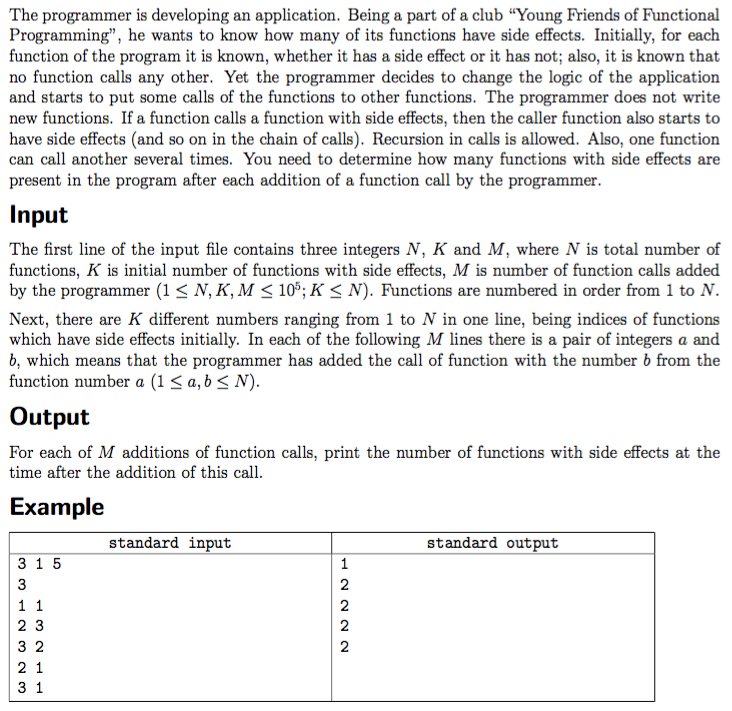
\includegraphics[width=0.9\textwidth]{OC_Siberia/L.png}\\ [1cm]
\end{center}

\textbf{{\large Алгоритм}}

Эту задачу можно решить поиском в ширину в графе вызовов функций, чтобы найти все зависимости в вызовах. Сложность алгоритма $O(N + M)$. \\

\newpage
\textbf{{\large Исходный код}} \\
\begin{lstlisting}[language=C++]
#include <iostream>
#include <vector>
#include <queue>
using namespace std;
int main(int argc, const char * argv[]) {
    int n, k, m;
    cin >> n >> k >> m;
    vector< vector<int> > g(n + 1, vector<int>());
    vector<bool> side_effect(n + 1, false);
    int func_num;
    for (int i = 0; i < k; i++) {
        cin >> func_num;
        side_effect[func_num] = true;
    }
    int a, b;
    int count = k;
    for (int i = 0; i < m; i++) {
        cin >> a >> b;
        g[b].push_back(a);
        if (!side_effect[a] && side_effect[b]) {
            side_effect[a] = true;
            count++;
            queue<int> q;
            q.push(a);
            vector<bool> used(n + 1);
            used[a] = true;
            while (!q.empty()) {
                int v = q.front();
                q.pop();
                for (size_t i = 0; i < g[v].size(); ++i) {
                    int to = g[v][i];
                    if (!used[to]) {
                        used[to] = true;
                        if (!side_effect[to]) {
                            side_effect[to] = true;
                            count++;
                            q.push(to);
                        }
                        
                    }
                }
            }
        }
        cout << count << endl;
    }
    return 0;
}
\end{lstlisting}








%----------------------------------------------------------------------------------------
%
%	OpenCup GrandPrix of Europe
%
%----------------------------------------------------------------------------------------
\newpage
\subsection{OpenCup GrandPrix of Europe}

\textbf{{\large Результаты}} \\
\begin{center}
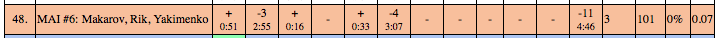
\includegraphics[width=0.95\textwidth]{OC_Europe/result.png}\\ [1cm]
\end{center}

\textbf{{\large Ссылка на контест: \url{http://opentrains.snarknews.info/~ejudge/team.cgi?contest_id=10327}}}

\newpage
\textbf{{\large Задача A - ASCII Addition}}

\begin{center}
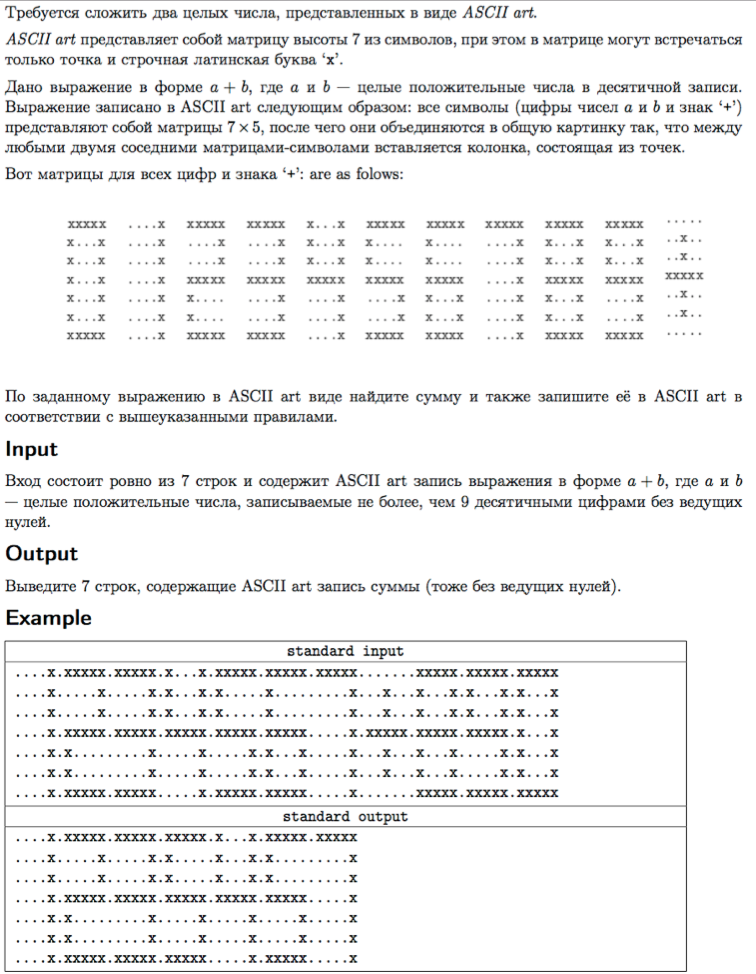
\includegraphics[width=0.9\textwidth]{OC_Europe/A.png}\\ [1cm]
\end{center}

\textbf{{\large Алгоритм}}

Задача просто на реализацию. \\

\newpage
\textbf{{\large Исходный код}} \\
\begin{lstlisting}[language=Perl]
my %digits = (
	"xxxxx".
	"x...x".
	"x...x".
	"x...x".
	"x...x".
	"x...x".
	"xxxxx" => 0,
	"....x".
	"....x".
	"....x".
	"....x".
	"....x".
	"....x".
	"....x" => 1,

	"xxxxx".
	"....x".
	"....x".
	"xxxxx".
	"x....".
	"x....".
	"xxxxx" => 2,

	"xxxxx".
	"....x".
	"....x".
	"xxxxx".
	"....x".
	"....x".
	"xxxxx" => 3,

	"x...x".
	"x...x".
	"x...x".
	"xxxxx".
	"....x".
	"....x".
	"....x" => 4,

	"xxxxx".
	"x....".
	"x....".
	"xxxxx".
	"....x".
	"....x".
	"xxxxx" => 5,

	"xxxxx".
	"x....".
	"x....".
	"xxxxx".
	"x...x".
	"x...x".
	"xxxxx" => 6,

	"xxxxx".
	"....x".
	"....x".
	"....x".
	"....x".
	"....x".
	"....x" => 7,

	"xxxxx".
	"x...x".
	"x...x".
	"xxxxx".
	"x...x".
	"x...x".
	"xxxxx" => 8,

	"xxxxx".
	"x...x".
	"x...x".
	"xxxxx".
	"....x".
	"....x".
	"xxxxx" => 9,

	".....".
	"..x..".
	"..x..".
	"xxxxx".
	"..x..".
	"..x..".
	"....." => "+"
	);
my %dig;
foreach my $key (keys %digits) {
	$dig{$digits{$key}} = $key;
}
my @screen;
for (my $i = 0; $i < 7; ++$i) {
	my $str = <>;
	chomp $str;
	my $n = length($str)+1;
	my $dig_cnt = $n/6;
	for (my $j = 0; $j < $dig_cnt; ++$j) {
		my $a = substr substr($str, $j*6, 6), 0, 5;
		$screen[$j] .= $a;
	}
}
my $expr = "";
foreach my $s (@screen) {
	$expr .= $digits{$s};
}
my $res = eval $expr;
for (my $i = 0; $i < 7; ++$i) {
	my $str = "";
	foreach my $d (split "", $res) {
		my $a = substr $dig{$d}, $i*5, 5;
		$str .= $a.".";
	}
	chop $str;
	print $str, "\n";
}
\end{lstlisting}


\newpage
\textbf{{\large Задача C - Counting Cities}}

\begin{center}
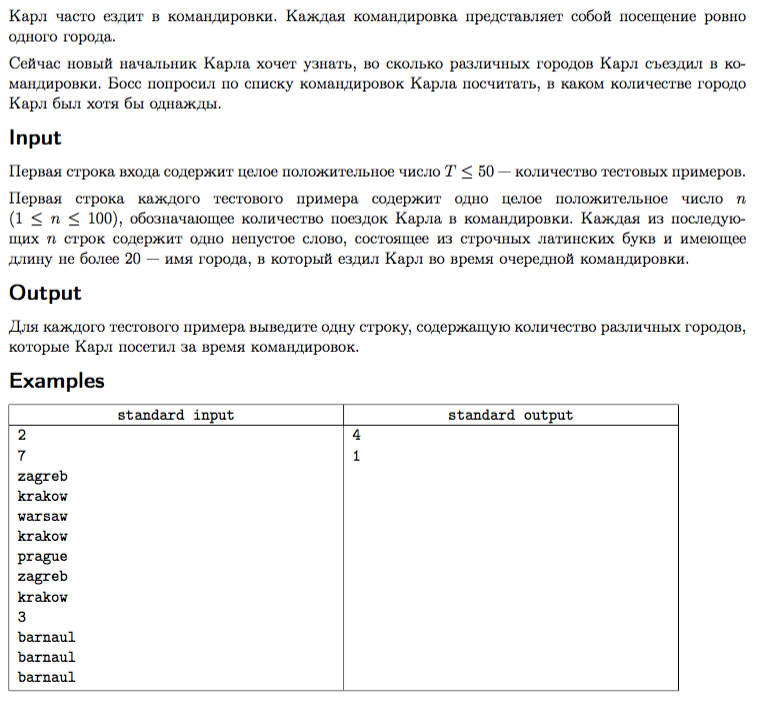
\includegraphics[width=0.9\textwidth]{OC_Europe/C.png}\\ [1cm]
\end{center}

\textbf{{\large Алгоритм}}

В этой задаче надо посчитать количество уникальных посещенных городов. Для этого каждую входную строку будем помещать в std::set, а потом просто выведем размер множества. \\

\newpage
\textbf{{\large Исходный код}} \\
\begin{lstlisting}[language=C++]
#include <iostream>
#include <set>
#include <string>

using namespace std;

int main(int argc, const char * argv[]) {
    
    int t;
    cin >> t;
    set<string> s;
    while (t--) {
        int n;
        cin >> n;
        string name;
        for (int i = 0; i < n; i++) {
            cin >> name;
            s.insert(name);
        }
        cout << s.size() << endl;
        s.clear();
    }
    
    return 0;
}

\end{lstlisting}


\newpage
\textbf{{\large Задача E - Electoral Estimations}}

\begin{center}
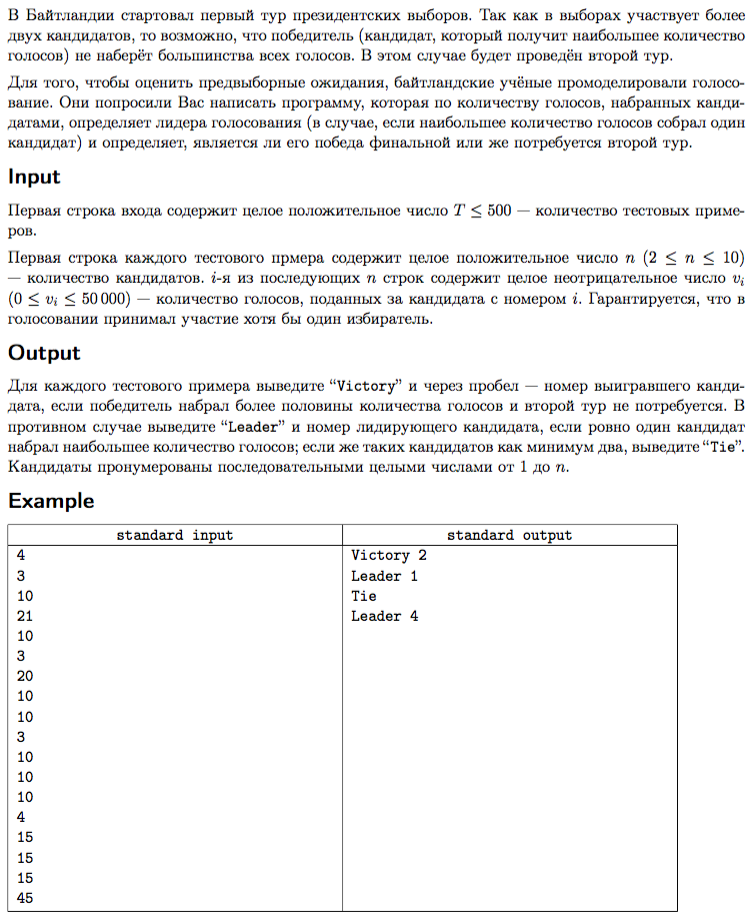
\includegraphics[width=0.9\textwidth]{OC_Europe/E.png}\\ [1cm]
\end{center}

\textbf{{\large Алгоритм}}

Для решения этой задачи нужно подсчитать голоса для каждого кандидата, отсортировать их и затем найти отношения количества голосов за победителя к остальным, чтобы определить, является он абсолютным победителем или нет. \\

\newpage
\textbf{{\large Исходный код}} \\
\begin{lstlisting}[language=C++]
#include <iostream>
#include <algorithm>
#include <vector>
typedef struct {
    int number;
    int votes;
} Person;
bool cmp(const Person &a, const Person &b) {
    return a.votes > b.votes;
}
using namespace std;
int main(int argc, const char * argv[]) {
    int t;
    cin >> t; 
    while (t--) {
        int n;
        cin >> n;
        int total_votes = 0;
        vector<Person> persons(n);
        for (int i = 0; i < n; i++) {
            persons[i].number = i + 1;
            cin >> persons[i].votes;
            total_votes += persons[i].votes;
        }
        sort(persons.begin(), persons.end(), cmp);
        int top_votes = persons[0].votes;
        int half_votes = total_votes / 2;
        if (t == 1) {
            cout << " " << endl;
        }
        if (top_votes > half_votes) {
            if (persons[1].votes != top_votes) {
                cout << "Victory " << persons[0].number << endl;
            } else {
                cout << "Tie" << endl;
            }
        } else {
            if (persons[1].votes != top_votes) {
                cout << "Leader " << persons[0].number << endl;
            } else {
                cout << "Tie" << endl;
            }
        }
    }
    return 0;
}
\end{lstlisting}






%----------------------------------------------------------------------------------------
%
%	OpenCup GrandPrix of Peterhof
%
%----------------------------------------------------------------------------------------
\newpage
\subsection{OpenCup GrandPrix of Peterhof}

\textbf{{\large Результаты}} \\
\begin{center}
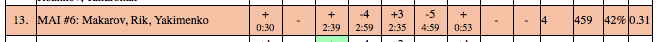
\includegraphics[width=0.95\textwidth]{OC_Peterhof/result.png}\\ [1cm]
\end{center}

\textbf{{\large Ссылка на контест: \url{http://opentrains.snarknews.info/~ejudge/team.cgi?contest_id=10328}}}

\newpage
\textbf{{\large Задача A - (a, b)-башня}}

\begin{center}
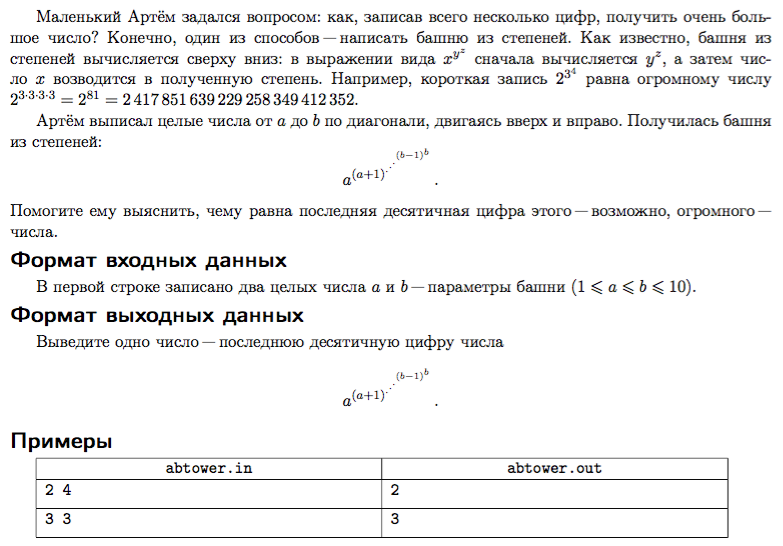
\includegraphics[width=0.9\textwidth]{OC_Peterhof/A.png}\\ [1cm]
\end{center}

\textbf{{\large Алгоритм}}

Задача решается с помощью рекурсии. Для того, чтобы узнать последнюю цифру конечного числа, на каждом шаге рекурсии можно отбрасывать все кроме последней цифры промежуточного числа. \\

\textbf{{\large Исходный код}} \\
\begin{lstlisting}[language=Ruby]
#!/usr/bin/env ruby
def func(l, r)
  if l < r
    (l ** func(l+1, r))%10
  else
    r%10
  end
end
a, b = gets.split.map {|x| x.to_i}
puts func(a,b)

\end{lstlisting}


\newpage
\textbf{{\large Задача C - Отношение эквивалентности}}

\begin{center}
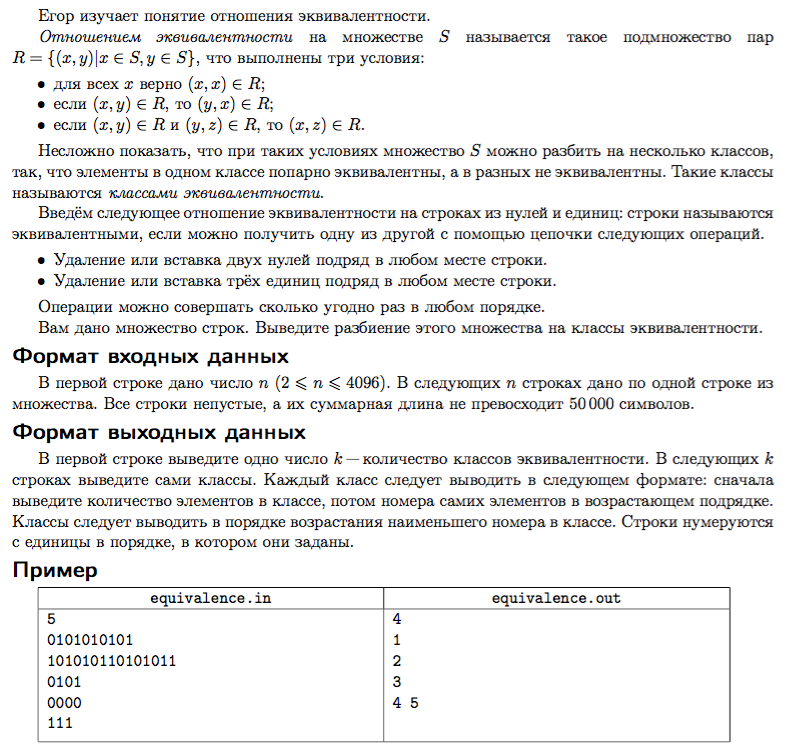
\includegraphics[width=0.9\textwidth]{OC_Peterhof/C.png}\\ [1cm]
\end{center}

\textbf{{\large Алгоритм}}

Задача на реализацию. Необходимо найти классы эквивалентности. \\

\textbf{{\large Исходный код}} \\
\begin{lstlisting}[language=Ruby]
n = gets.to_i

data = Array.new

for i in 0...n
    s = gets.chomp
    data.push(s)
end

data.each do |s|
    begin
        s_copy = s.clone
        s.gsub!(/0{2}/,'')
        s.gsub!(/1{3}/,'')
    end until s == s_copy
end

h = Hash.new()

data.each_index do |i|
    s = data[i]
    if h[s] == nil
        h[s] = Array.new
    end
    h[s].push(i + 1)
end

res = Array.new

h.each_value do |v|
    res.push(v)
end

res.sort! do |a, b|
    a.first <=> b.first
end

puts "#{res.size}"

res.each do |l|
    l.each do |x|
        print "#{x} "
    end
    puts
end

\end{lstlisting}

\newpage
\textbf{{\large Задача E - Идеальная фотография}}

\begin{center}
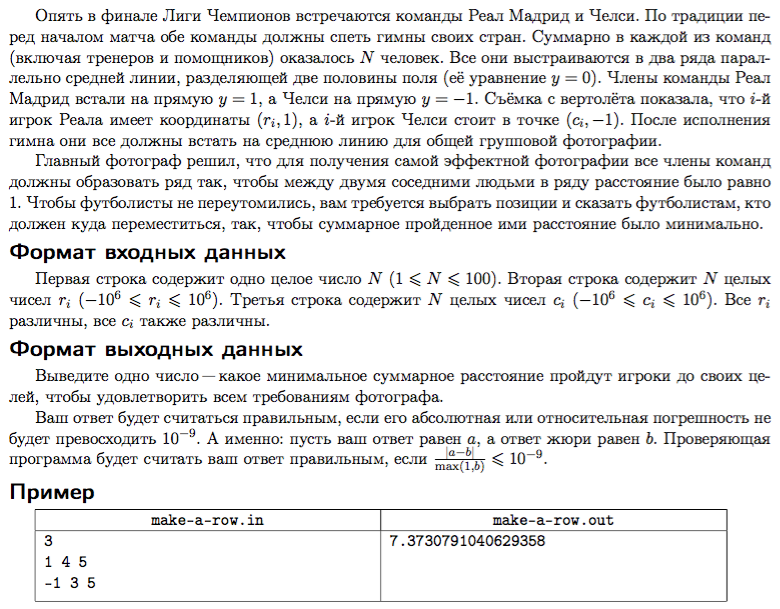
\includegraphics[width=0.9\textwidth]{OC_Peterhof/E.png}\\ [1cm]
\end{center}

\textbf{{\large Алгоритм}}

Нужно единожды выстроить всех людей в одну линию по порядку и потом двигать эту линию, пока растояние не станет наименьшим с заданной точностью. \\

\newpage
\textbf{{\large Исходный код}} \\
\begin{lstlisting}[language=Ruby]
#!/usr/bin/env ruby
def calc_sum(m, i)
  s = 0
  for a in m do
    s += Math.sqrt((a-i)*(a-i) + 1)
    i += 1
  end
  return s
end
n = gets.to_i
r = gets.split.map{|x| x.to_i}
c = gets.split.map{|x| x.to_i}
m = (r + c).sort
x = 0
step = 1000000
sum_curr = calc_sum(m, x)
sum_prev = sum_curr + 1
sign = 1
x += step
while ((sum_prev-sum_curr).abs > 0.0000000001)
  sum_prev = sum_curr
  sum_curr = calc_sum(m, x)
  if sum_curr > sum_prev && sign == 1
    sign = -1
    step /= 2.0
    sign_counter = 0
  elsif sum_curr > sum_prev && sign == -1
     sign = 1
     step /= 2.0
     sign_counter = 0
  end
  x += step*sign
end
puts sum_curr

\end{lstlisting}

\newpage
\textbf{{\large Задача G - Случайные тоннели}}

\begin{center}
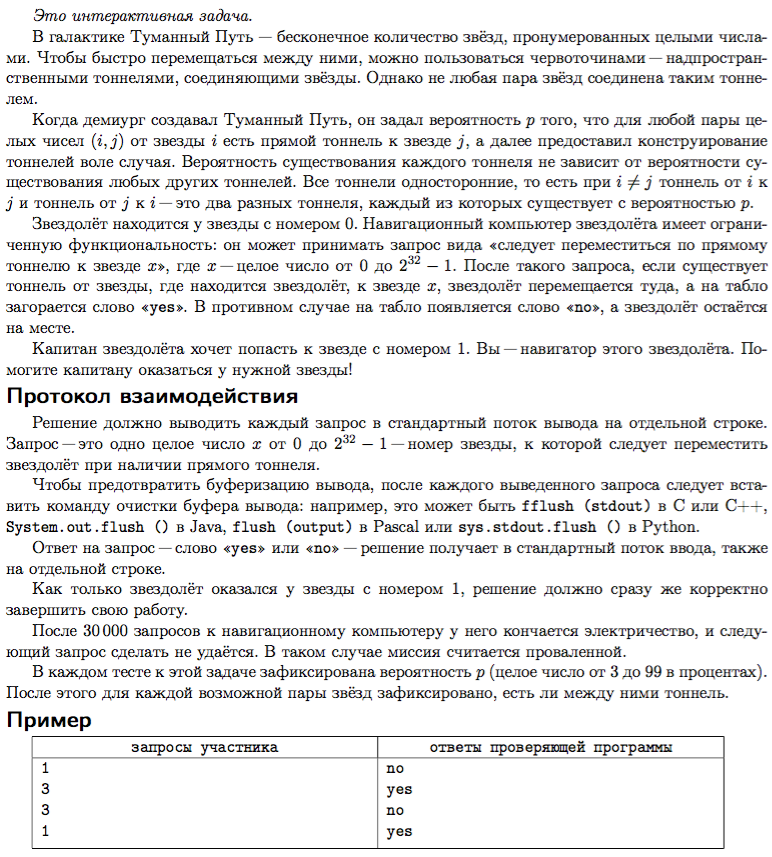
\includegraphics[width=0.9\textwidth]{OC_Peterhof/G.png}\\ [1cm]
\end{center}

\textbf{{\large Алгоритм}}

Для выбора следующей звезды можно использовать случайные числа и при успешном перемещении на эту звезду нужно проверить, существует ли путь до звезды 1, если нет, то повторить алгоритм сначала. \\

\newpage
\textbf{{\large Исходный код}} \\
\begin{lstlisting}[language=Ruby]
#!/usr/bin/env ruby
def send_cmd(cmd)
  puts cmd
  STDOUT.flush
end
a = 1
while (true) do
  send_cmd a
  case gets
  when /yes/
    exit if a == 1
    a = 1
  when /no/
    a = rand(1<<31)
  end
end

\end{lstlisting}






%----------------------------------------------------------------------------------------
%
%	OpenCup Grand Prix of Asia
%
%----------------------------------------------------------------------------------------
\newpage
\subsection{OpenCup Grand Prix of Asia}

\textbf{{\large Результаты}} \\
\begin{center}
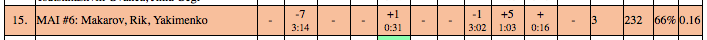
\includegraphics[width=0.95\textwidth]{OC_Asia/result.png}\\ [1cm]
\end{center}

\textbf{{\large Ссылка на контест: \url{http://opentrains.snarknews.info/~ejudge/team.cgi?contest_id=10329}}}

\newpage
\textbf{{\large Задача E - Mirror Rice Cake}}

\begin{center}
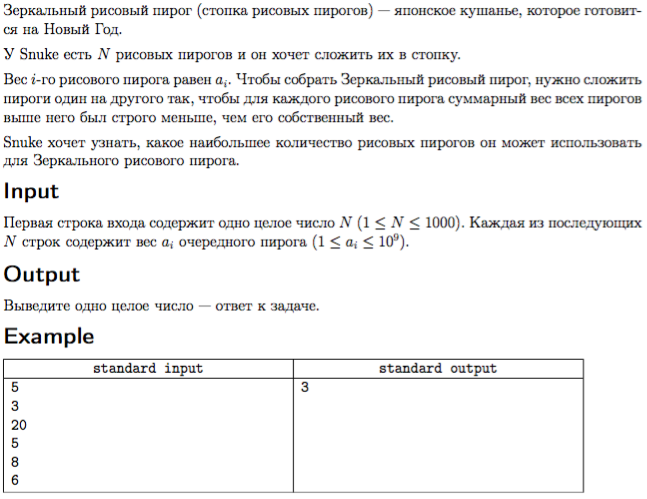
\includegraphics[width=0.9\textwidth]{OC_Asia/E.png}\\ [1cm]
\end{center}

\textbf{{\large Алгоритм}}

Сортируем и складываем все числа до тех пор, пока общая сумма не станет больше следующего слагаемого. \\
\newpage
\textbf{{\large Исходный код}} \\
\begin{lstlisting}[language=Java]
import java.util.*;
public class Test {
    public static void main(String[] args) {        
      Scanner sc = new Scanner(System.in);
      int N = sc.nextInt();      
      long a[] = new long[N];      
      for(int i = 0; i < N; i++) {
          a[i] = sc.nextInt();
      }
      int count = 1;
      Arrays.sort(a);
      long sum = a[0];
      for(int i = 1; i < N; i++) {
          if(a[i] > sum) {
              count++;
              sum += a[i];
          }
      }
      System.out.println(count);      
    }
}
\end{lstlisting}


\newpage
\textbf{{\large Задача L - String Modifcation}}

\begin{center}
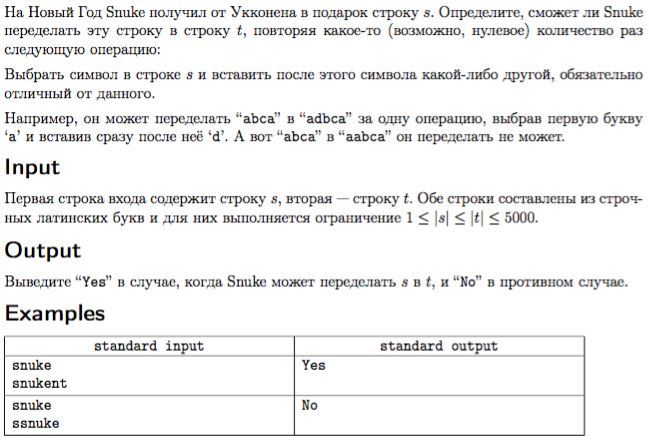
\includegraphics[width=0.9\textwidth]{OC_Asia/L.png}\\ [1cm]
\end{center}

\textbf{{\large Алгоритм}}

Задача на реализацию. \\
\newpage
\textbf{{\large Исходный код}} \\
\begin{lstlisting}[language=Ruby]
#!/usr/bin/env ruby
a = gets.chomp
b = gets.chomp
i = 0
j = 0
f = false
fc = b[0]
while j < b.length do
  if fc != b[j]
    f = true
  end
  if i < a.length && a[i] == b[j]
    i += 1
    j += 1
  elsif i == 0
    puts 'No'
    exit
  else
    if b[j-1] == b[j] && !f
      puts 'No'
      exit
    end
    j += 1
  end
end
if i == a.length
  puts 'Yes'
else
  puts 'No'
end
\end{lstlisting}


\newpage
\textbf{{\large Задача N - Soccer Match}}

\begin{center}
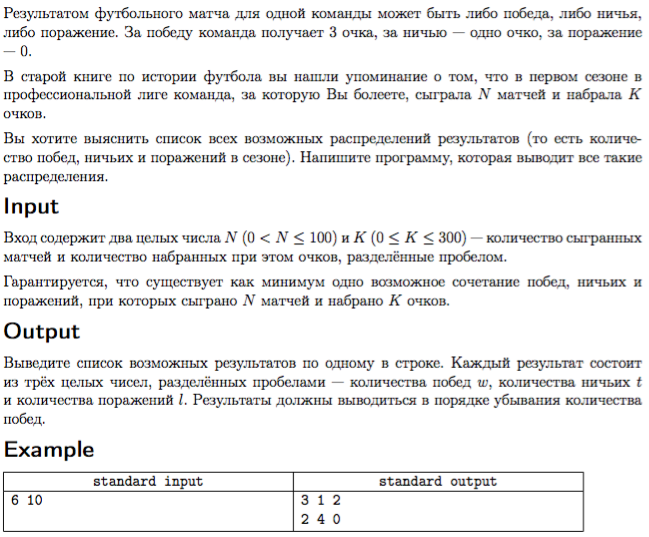
\includegraphics[width=0.9\textwidth]{OC_Asia/N.png}\\ [1cm]
\end{center}

\textbf{{\large Алгоритм}}

Перебор всех возможных варинтов с использованием формул. Сложность $O(n)$. \\

\textbf{{\large Исходный код}} \\
\begin{lstlisting}[language=Ruby]
input = gets.split(' ').map(&:to_i)
games = input.first
score = input.last
wins = score / 3
ties = 0
losses = 0
while wins > games
    wins = wins - 1
end
while wins > -1
    ties = score - wins * 3
    losses = games - wins - ties
    break if ties < 0 or losses < 0
    puts "#{wins} #{ties} #{losses}"
    wins = wins - 1
end
\end{lstlisting}






%----------------------------------------------------------------------------------------
%
%	OpenCup GrandPrix of Saratov
%
%----------------------------------------------------------------------------------------
\newpage
\subsection{OpenCup GrandPrix of Saratov}

\textbf{{\large Результаты}} \\
\begin{center}
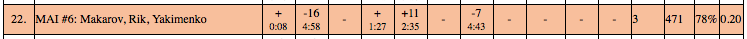
\includegraphics[width=0.95\textwidth]{OC_Saratov/result.png}\\ [1cm]
\end{center}

\textbf{{\large Ссылка на контест: \url{hhttp://opentrains.snarknews.info/~ejudge/team.cgi?contest_id=10340}}}

\newpage
\textbf{{\large Задача A - Алфавит}}

\begin{center}
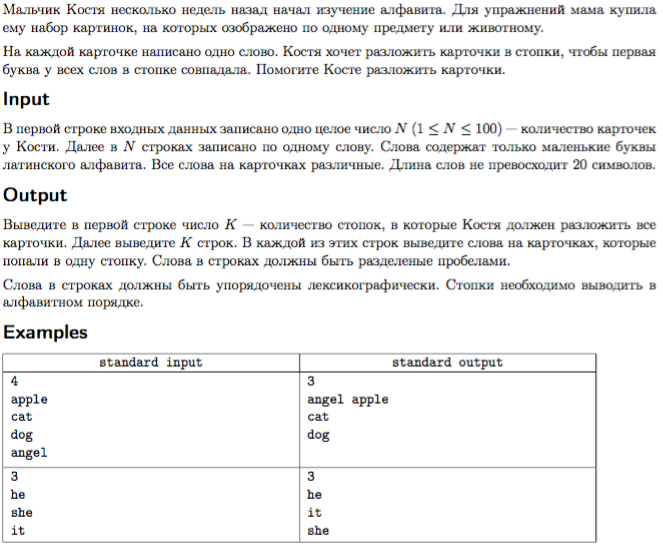
\includegraphics[width=0.9\textwidth]{OC_Saratov/A.png}\\ [1cm]
\end{center}

\textbf{{\large Алгоритм}}

Группируем все слова по первой букве с помощью ассоциативного массива и затем выводим в отсортированном виде. \\

\textbf{{\large Исходный код}} \\
\begin{lstlisting}[language=Ruby]
n = gets.chomp.to_i
h = {}
for i in 0...n
  word = gets.chomp
  c = word[0]
  unless h.has_key?(c)
    h[c] = []
  end
  h[c].push(word)
end
puts h.size
for a in h.keys.sort
  puts h[a].sort.join(' ')
end
\end{lstlisting}


\newpage
\textbf{{\large Задача D - Возрастающие последовательности}}

\begin{center}
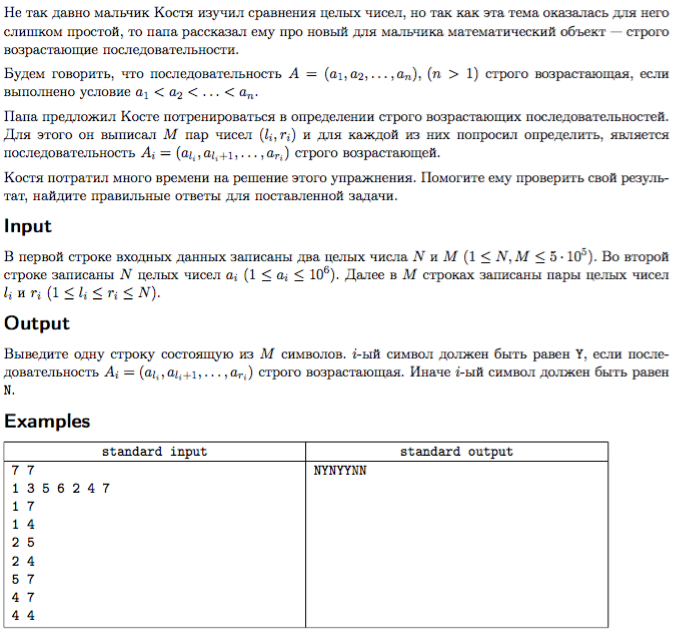
\includegraphics[width=0.9\textwidth]{OC_Saratov/D.png}\\ [1cm]
\end{center}

\textbf{{\large Алгоритм}}

Задача решается простым перебором. Сложность $O(n)$. \\

\textbf{{\large Исходный код}} \\
\begin{lstlisting}[language=C++]
#include <iostream>
#include <algorithm>
#include <vector>
#include <cmath>
#include <set>
#include <string>
#define LL long long
#define ULL  unsigned long long
using namespace std;
ULL myAbs(ULL a, ULL b) {
	if(a > b) {
		return a - b;
	} else {
		return b - a + 1;
	}
}
typedef struct {
	int first;
	int second;
	int d;
} dist;

bool comp(const dist &a, const dist &b) {
    return a.d > b.d;
}
int main() {

	int temp;
	
	int N, M;
	cin >> N >> M;

	vector <int> up(N, 0);
	int cur, prev;
	cin >> prev;
	int k = 0;

	for(int i = 1; i < N; i++) {
		cin >> cur;
		if(cur > prev) {
			up[i] = k;
		}
		else {
			k++;
			up[i] = k;
		}
		prev = cur;
	}

	int l, r;
	for(int i = 0; i < M; i++) {
		cin >> l >> r;
		if(up[l-1] == up[r-1] && l != r) {
			cout << "Y";
		}
		else {
			cout << "N";
		}
	}

	//cin >> temp;
	
	return 0;

}
\end{lstlisting}


\newpage
\textbf{{\large Задача E - Карточки}}

\begin{center}
\includegraphics[width=0.9\textwidth]{OC_Saratov/E.png}\\ [1cm]
\end{center}

\textbf{{\large Алгоритм}}

Задача решается с помощью перебора. \\
\newpage
\textbf{{\large Исходный код}} \\
\begin{lstlisting}[language=C++]
#include <iostream>
#include <algorithm>
#include <vector>
#include <set>
using namespace std;

int main() {
  long n;
  cin >> n;
  vector<long> a(n);
  for (long i = 0; i < n; ++i) {
    long d;
    cin >> d;
    a[i] = d;
  }
  sort(a.begin(), a.end());
  set<long> h;
  long max_s = 1;
  for (long i = 0; i < n; ++i) {
    long j = n-1;
    while (j > i) {
      if (j-i <= 2 * max_s)
        break;
      long sum = a[i] + a[j];
      if (h.find(sum) != h.end()) {
        j -= 1;
        continue;
      }
      else {
        h.insert(sum);
      }
      long count = 1;
      long y = j-1;
      for (long k = i+1; k <= y; ++k) {
        bool f = false;
        long x = y;
        while (!f && x > k) {
          long sum_k = a[k] + a[x];
          if (sum_k == sum) {
            count += 1;
            y = x - 1;
            f = true;
          }
          else if (sum_k < sum) {
            break;
          }
          x -= 1;
        }
      }
      if (count > max_s) {
        max_s = count;
      }
      j -= 1;
    }
  }
  cout << max_s << '\n';
  return 0;
}

\end{lstlisting}






%----------------------------------------------------------------------------------------
%
%	OpenCup GrandPrix of China
%
%----------------------------------------------------------------------------------------
\newpage
\subsection{OpenCup GrandPrix of China}

\textbf{{\large Результаты}} \\
\begin{center}
\includegraphics[width=0.95\textwidth]{OC_China_2016/result.png}\\ [1cm]
\end{center}

\textbf{{\large Ссылка на контест: \url{http://opentrains.snarknews.info/~ejudge/team.cgi?contest_id=10341}}}

\newpage
\textbf{{\large Задача L - Cut The Rectangle}}

\begin{center}
\includegraphics[width=0.9\textwidth]{OC_China_2016/L.png}\\ [1cm]
\end{center}

\textbf{{\large Алгоритм}}

Для решения задачи нужно просто проверить равенство треуголника. Сложность $O(1))$. \\

\textbf{{\large Исходный код}} \\
\begin{lstlisting}[language=Ruby]
a = gets.split(' ').map(&:to_i)
b = gets.split(' ').map(&:to_i)
as = a.sort.join('')
bs = b.sort.join('')
if (a[0]**2 + a[1]**2 == a[2]**2 ||
  a[0]**2 + a[2]**2 == a[1]**2 ||
  a[2]**2 + a[1]**2 == a[0]**2 &&
  as == bs)
  puts 1
else
  puts 0
end
\end{lstlisting}


\newpage
\textbf{{\large Задача M - Diversity}}

\begin{center}
\includegraphics[width=0.9\textwidth]{OC_China_2016/M.png}\\ [1cm]
\end{center}

\textbf{{\large Алгоритм}}

Нужно удалять из слова буквы, которых меньше всего, до тех пор, пока различных букв не станет 1 или 2 штуки. \\

\textbf{{\large Исходный код}} \\
\begin{lstlisting}[language=Ruby]
aa = gets.chomp
h = {}
count = 0
for i in 0...a.size
  if h.has_key?(a[i])
    h[a[i]] += 1
  else
    h[a[i]] = 1
    count += 1
  end
end
if count <= 2
  puts 0
else
  m = h.values.sort
  sum = 0
  n = m.size - 2
  for i in 0...n
    sum += m[i]
  end
  puts sum
end
\end{lstlisting}


\newpage
\textbf{{\large Задача N - Mechanics}}

\begin{center}
\includegraphics[width=0.9\textwidth]{OC_China_2016/N_1.png}\\
\includegraphics[width=0.9\textwidth]{OC_China_2016/N_2.png}\\ [1cm]
\end{center}

\textbf{{\large Алгоритм}}

Задача на реализацию. Нужно учитывать, что если соединения колёс от первого к последним образуют дерево, то колёса могут крутиться, и направление у колёс чередуется. Также, для подсчёта частоты вращения требуется сокращать дробь на каждом шаге.  \\

\textbf{{\large Исходный код}} \\
\begin{lstlisting}[language=C++]
#include <iostream>
#include <vector>
#include <cmath>
#include <queue>
using namespace std;
#define ll long long
#define ull unsigned long long
#define eps 0.0000000001
struct Gear {
  ll x, y, r;
  bool f;
  char sign;
  ll a, b;
  vector<ll> list;
  ll parent;
  Gear(ll a, ll b, ll c) {
    x = a;
    y = b;
    r = c;
    f = 0;
  }
};

double eq_eps(double a, double b) {
  return fabs(a - b) < eps;
}

int main() {
  ll n;
  cin >> n;
  vector<Gear *> v(n);
  for (int i = 0; i < n; ++i) {
    ll a, b, c;
    cin >> a >> b >> c;
    v[i] = new Gear(a, b, c);
  }
  for (int i = 0; i < n; ++i) {
    for (int j = i+1; j < n; ++j) {
      bool res = eq_eps(sqrt(pow(v[i]->x - v[j]->x, 2) + pow(v[i]->y - v[j]->y, 2)), v[i]->r + v[j]->r);
      if (res) {
        v[i]->list.push_back(j);
        v[j]->list.push_back(i);
      }

    }
  }
  ll x = 0;
  v[x]->a = 1;
  v[x]->b = 1;
  v[x]->sign = 1;
  queue<ll> qu;
  qu.push(x);
  while (!qu.empty()) {
    x = qu.front();
    qu.pop();
    Gear * cur_gear = v[x];
    for (ll i = 0; i < cur_gear->list.size(); ++i) {
      if (cur_gear->list[i] == cur_gear->parent)
        continue;
      Gear * next_gear = v[cur_gear->list[i]];
      if (!next_gear->f) {
        qu.push(cur_gear->list[i]);
        next_gear->f = 1;
        next_gear->parent = x;
      }
      else {
        cout << -1 << endl;
        return 0;
      }
      next_gear->sign = cur_gear->sign * -1;
      ll new_a, new_b, a, b;
      a = new_a = cur_gear->r * cur_gear->a;
      b = new_b = next_gear->r * cur_gear->b;
      while (b != 0) {
          ll r = a%b;
          a = b; b = r;
      }
      next_gear->a = new_a/a;
      next_gear->b = new_b/a;
    }
  }
  Gear * last_gear = v[n-1];
  if (last_gear->f == 0) {
    cout << 0 << endl;
    return 0;
  }
  ll a = last_gear->a;
  ll b = last_gear->b;
  while (b != 0) {
      ll r = a%b;
      a = b; b = r;
  }
  cout << last_gear->b/a << ' ' << last_gear->sign * last_gear->a/a << endl;

  return 0;
}
\end{lstlisting}


\newpage
\textbf{{\large Задача O - Pairs}}

\begin{center}
\includegraphics[width=0.9\textwidth]{OC_China_2016/O.png}\\ [1cm]
\end{center}

\textbf{{\large Алгоритм}}

Задача на реализацию. \\

\textbf{{\large Исходный код}} \\
\begin{lstlisting}[language=C++]
#include <iostream>
#include <algorithm>
#include <vector>
using namespace std;
typedef struct {
    long suit;
    long cost;
    int id;
} Card;
bool cmp_suit(const Card &a, const Card &b)
{
    return a.suit < b.suit;
}
bool cmp_cost(const Card &a, const Card &b)
{
    return a.cost < b.cost;
}
int main()
{
    int n;
    cin >> n;
    vector<Card> hand(n);
    for (int i = 0; i < n; i++) {
        cin >> hand[i].suit >> hand[i].cost;
        hand[i].id = i + 1;
    }
    stable_sort(hand.begin(), hand.end(), cmp_cost);
    stable_sort(hand.begin(), hand.end(), cmp_suit);
    vector< pair<int, int> > output;
    vector< vector<int> > jazz;
    for (int i = 1; i <= n; i++) {
        vector<int> temp;
        temp.push_back(hand[i - 1].id);
        while (i < n && hand[i].suit == hand[i - 1].suit) {
            temp.push_back(hand[i].id);
            i++;
        }
        jazz.push_back(temp);
    }
    for (size_t i = 0; i < jazz.size(); i++) {
        if (jazz[i].size() < 2) {
            cout << "-1" << endl;
            return 0;
        } else {
            output.push_back(make_pair(jazz[i][0], jazz[i][1]));
        }
    }
    cout << output.size() << endl;
    for (size_t i = 0; i < output.size(); i++) {
        cout << output[i].first << " " << output[i].second << endl;
    }
    return 0;
}
\end{lstlisting}






%----------------------------------------------------------------------------------------
%
%	OpenCup GrandPrix of Bashkortostan
%
%----------------------------------------------------------------------------------------
\newpage
\subsection{OpenCup GrandPrix of Bashkortostan}

\textbf{{\large Результаты}} \\
\begin{center}
\includegraphics[width=0.95\textwidth]{OC_Bashkortostan/result.png}\\ [1cm]
\end{center}

\textbf{{\large Ссылка на контест: \url{http://opentrains.snarknews.info/~ejudge/team.cgi?contest_id=10342}}}

\newpage
\textbf{{\large Задача C - Constant Ratio}}

\begin{center}
\includegraphics[width=0.9\textwidth]{OC_Bashkortostan/C.png}\\ [1cm]
\end{center}

\textbf{{\large Алгоритм}}

Задача решается перебором. \\

\textbf{{\large Исходный код}} \\
\begin{lstlisting}[language=C++]
#include <stdio.h>
#include <math.h>

int main()
{
    long x;
    scanf("%ld", &x); 
    long count = 0; 
    long d;
    for (d = 1; d < x; d++) {
        if (x % d == 0) {
            count++;
        }
    } 
    long b1, q, n;
    for (b1 = 1; b1 <= (x/3 + 1); b1++)
    {
        long q_max = ceil((double)x / b1) - 1;     
        for (q = 2; q <= q_max; q++)
        {
            for (n = 2; n <= 100000; n++)
            {
                long s = (b1 * ((long)pow((double)q, (double)n) - 1)) / (q - 1);
                if (s == x) {
                    count++;
                } else if (s > x) {
                    break;
                }
            }
        }
    }   
    printf("%ld\n", count);  
    return 0;
}
\end{lstlisting}


\newpage
\textbf{{\large Задача L - Игра со строкой}}

\begin{center}
\includegraphics[width=0.9\textwidth]{OC_Bashkortostan/L.png}\\ [1cm]
\end{center}

\textbf{{\large Алгоритм}}

Задача решается с помощью конечного автомата, полученного при исследовании поведения строки при различных входных данных. \\

\textbf{{\large Исходный код}} \\
\begin{lstlisting}[language=Ruby]
n = gets.to_i
counter = 0
state = 'a'
a = n
while a > 1
  if state == 'a'
    if a&1 == 1
      state = 'c'
    else
      state = 'b'
    end
    counter += (a.to_f / 2.0).ceil
  elsif state == 'b'
    d = a / 2
    counter += d
    a -= d
    state = 'a'
  else
    state = 'a'
    d = (a.to_f / 2.0).ceil
    counter += d
    a += d
  end
end
puts counter
\end{lstlisting}


\newpage
\textbf{{\large Задача N - Numbers}}

\begin{center}
\includegraphics[width=0.9\textwidth]{OC_Bashkortostan/N.png}\\ [1cm]
\end{center}

\textbf{{\large Алгоритм}}

Задача на реализацию. \\
\newpage
\textbf{{\large Исходный код}} \\
\begin{lstlisting}[language=Ruby]
t = gets.to_i

t.times do
    inp = gets.split(' ').map(&:to_i)

    n = inp.first
    x = inp.last

    first_class = true
    if n % 4 == 0 or (n + 1) % 4 == 0
        first_class = false
    end

    nums = []

    if first_class
        #nums = (1..n).step(2).to_a
        if !x.even? and x <= n
            puts 'YES'
        else
            puts 'NO'
        end
    else
        #nums = (0..n).step(2).to_a
        if x.even? and x <= n
            puts 'YES'
        else
            puts 'NO'
        end
    end
end
\end{lstlisting}


\newpage
\textbf{{\large Задача O - Ones as the Difference}}

\begin{center}
\includegraphics[width=0.9\textwidth]{OC_Bashkortostan/O.png}\\ [1cm]
\end{center}

\textbf{{\large Алгоритм}}

Генерируем все варианты ответов с помощью перебора и вставляем в код конечной программы. \\
\newpage
\textbf{{\large Исходный код}} \\
Генератор:
\begin{lstlisting}[language=Ruby]
n = gets.to_i

if n < 10
    puts n
else
    count = 9
    num = 10
    while true
        good_num = true
        num_as_str = num.to_s
        for i in 1...(num_as_str.size)
            digit_l = num_as_str[i - 1].to_i
            digit_r = num_as_str[i].to_i
            if (digit_r - digit_l).abs != 1
                good_num = false
                break
            end
        end
        if good_num
            count = count + 1
            print "#{num},"
        end
        if count == n
            puts num
            break
        end
        num = num + 1
    end
end
\end{lstlisting}
Программа с предподсчитанными числами:
\begin{lstlisting}[language=Ruby]
n = gets.to_i
answer = [1,2,3,4,5,...generated_numbers...,2123456,2123456]
puts answer[n - 1]
\end{lstlisting}


\newpage
\textbf{{\large Задача P - Places at the Olympics}}

\begin{center}
\includegraphics[width=0.9\textwidth]{OC_Bashkortostan/P.png}\\ [1cm]
\end{center}

\textbf{{\large Алгоритм}}

Задача на реализацию. \\
\newpage
\textbf{{\large Исходный код}} \\
\begin{lstlisting}[language=Ruby]
t = gets.to_i

t.times do
    medals = gets.split(' ').map(&:to_i)
    temp = medals.each_slice(3).to_a
    berland = temp.first
    byteland = temp.last
    # test Win
    berland_count = berland.inject(:+)
    byteland_count = byteland.inject(:+)
    count_win = false
    if (berland_count > byteland_count)
        count_win = true
    end
    # test Quality
    quality_win = false
    if berland[0] > byteland[0]
        quality_win = true
    elsif berland[0] == byteland[0] and
          berland[1] > byteland[1]
          quality_win = true
    elsif berland[0] == byteland[0] and
          berland[1] == byteland[1] and
          berland[2] > byteland[2]
          quality_win = true
    end
    if count_win and quality_win
        puts "Win"
    elsif count_win
        puts "Count"
    elsif quality_win
        puts "Quality"
    else
        puts "None"
    end
end
\end{lstlisting}



\newpage
\textbf{{\large Задача Q - Quaqua the Frog}}

\begin{center}
\includegraphics[width=0.9\textwidth]{OC_Bashkortostan/Q.png}\\ [1cm]
\end{center}

\textbf{{\large Алгоритм}}

Сложность $O(n^2)$. \\
\newpage
\textbf{{\large Исходный код}} \\
\begin{lstlisting}[language=Java]
import java.util.*;
public class Test {
    public static void main(String[] args) {        
      Scanner sc = new Scanner(System.in);
      int T = sc.nextInt();
      int c;
      int j;
      String s;      
      for(int i = 0; i < T; i++) {
          c = sc.nextInt();
          j = sc.nextInt();          
          char arr[];
          sc.nextLine();
          s = sc.nextLine();
          arr = s.toCharArray();
          boolean frogCan = false;
          int count = 0;
          int cur = 0;
          while(true) {
            if(cur + j + 1 < c - 1) {
                if(arr[cur+j + 1] == '.') {
                    cur += j + 1;
                    count++;
                    frogCan = true;
                } else {
                    for(int jTemp = j - 1; jTemp >= 0; jTemp--) {
                        if(arr[cur + jTemp + 1] == '.') {
                            cur += jTemp + 1;
                            count++;
                            frogCan = true;
                            break;
                        }
                    }
                }
                if(!frogCan) {
                    break;
                }
                frogCan = false;
            } else {
                count++;
                frogCan = true;
                break;
            }
        }
        if(!frogCan) {
             System.out.println("-1");
        } else {
             System.out.println(count);
        }           
      }    
    }
}
\end{lstlisting}



\newpage
\textbf{{\large Задача R - Road in Mountains}}

\begin{center}
\includegraphics[width=0.9\textwidth]{OC_Bashkortostan/R.png}\\ [1cm]
\end{center}

\textbf{{\large Алгоритм}}

Задача на реализацию. Сложность $O(n)$. \\
\newpage
\textbf{{\large Исходный код}} \\
\begin{lstlisting}[language=Java]
import java.util.*;
public class Test {
    public static void main(String[] args) {
      Scanner sc = new Scanner(System.in);
      int N = sc.nextInt();
      double temp;
      double S = 0;
      double t = 0;      
      double arr[][] = new double[N][2];
      for(int i = 0; i < N; i++) {
          temp = sc.nextDouble();
          arr[i][0] = temp;
          S += arr[i][0];    
          temp = sc.nextDouble();
          arr[i][1] = temp;
          t += arr[i][0] / arr[i][1];
      }
      System.out.println(S/t);
    }
}
\end{lstlisting}






%----------------------------------------------------------------------------------------
%
%	OpenCup GrandPrix of Tatarstan
%
%----------------------------------------------------------------------------------------
\newpage
\subsection{OpenCup GrandPrix of Tatarstan}

\textbf{{\large Результаты}} \\
\begin{center}
\includegraphics[width=0.95\textwidth]{OC_Tatarstan_2016/result.png}\\ [1cm]
\end{center}

\textbf{{\large Ссылка на контест: \url{http://opentrains.snarknews.info/~ejudge/team.cgi?contest_id=10344}}}

\newpage
\textbf{{\large Задача G - Кастрюли}}

\begin{center}
\includegraphics[width=0.9\textwidth]{OC_Tatarstan_2016/G.png}\\ [1cm]
\end{center}

\textbf{{\large Алгоритм}}

Подсчитываем количество каждого вида кастрюль и выбираем наибольшее. Сложность $O(n)$. \\

\textbf{{\large Исходный код}} \\
\begin{lstlisting}[language=Ruby]
n = gets.to_i
data = gets.split(' ').map(&:to_i)

h = Hash.new
data.each do |item|
    el = h[item]
    if el == nil
        h[item] = 1
    else
        h[item] = el + 1
    end
end

top = 0
h.each_value do |val|
    if val > top
        top = val
    end
end
puts top
\end{lstlisting}


\newpage
\textbf{{\large Задача M - Наименьшая дробь}}

\begin{center}
\includegraphics[width=0.9\textwidth]{OC_Tatarstan_2016/M.png}\\ [1cm]
\end{center}

\textbf{{\large Алгоритм}}

Задача решается с помощью итеративного вычисления наибольшого общего делителя и наименьшого общего множителя. Сложность $O(n)$. \\
\newpage
\textbf{{\large Исходный код}} \\
\begin{lstlisting}[language=Java]
import java.util.Scanner;
public class OpenCup {
    public static long gcd (long a, long b) {
	if (b == 0)
		return a;
	else
		return gcd (b, a % b);
    }
    public static long lcm (long a, long b) {
	return a / gcd (a, b) * b;
    }
    public static void main(String[] args) {
        Scanner in = new Scanner(System.in);
        int n = in.nextInt();
        long[] a = new long[n];
        long[] b = new long[n];
        for(int i = 0; i < n; i++) {
            a[i] = in.nextLong();
            b[i] = in.nextLong();            
        }
        long A = a[0], B = b[0];
        for(int i = 0; i < n - 1; i++) {
            b[i + 1] = gcd(b[i], b[i + 1]);
            a[i + 1] = lcm(a[i], a[i + 1]);
        }
        A = a[n - 1];
        B = b[n - 1];
        long t = gcd(A, B);
        A = A / t;
        B = B / t;
        System.out.println(A + " " + B);
    }
}
\end{lstlisting}






%----------------------------------------------------------------------------------------
%
%	OpenCup GrandPrix of Baltics
%
%----------------------------------------------------------------------------------------
\newpage
\subsection{OpenCup GrandPrix of Baltics}

\textbf{{\large Результаты}} \\
\begin{center}
\includegraphics[width=0.95\textwidth]{OC_Baltics/result.png}\\ [1cm]
\end{center}

\textbf{{\large Ссылка на контест: \url{http://opentrains.snarknews.info/~ejudge/team.cgi?contest_id=10344}}}

\newpage
\textbf{{\large Задача E - Поиск уникального элемента}}

\begin{center}
\includegraphics[width=0.9\textwidth]{OC_Baltics/E.png}\\ [1cm]
\end{center}

\textbf{{\large Алгоритм}}

Задача решается с помощью бинарного поиска. Сложность $O(log_2(n))$. \\
\newpage
\textbf{{\large Исходный код}} \\
\begin{lstlisting}[language=Ruby]
n = gets.to_i
if n == 1
    puts "? 1"
    STDOUT.flush
    puts "! #{gets}"
    STDOUT.flush
    exit
end
idx1 = 1
idx2 = 2
l = 1
r = n
a = 0
b = 0
while true
    idx1 = (l + r) / 2
    if idx1.even?
        idx1 = idx1 - 1
    end
    idx2 = idx1 + 1
    if idx2 > n or l == r
        puts "? #{idx1}"
        STDOUT.flush
        a = gets.to_i
        puts "! #{a}"
        STDOUT.flush
        exit
    end
    puts "? #{idx1}"
    STDOUT.flush
    a = gets.to_i
    puts "? #{idx2}"
    STDOUT.flush
    b = gets.to_i
    if a != b
        r = idx1
    else
        l = idx2 + 1
    end
end
\end{lstlisting}


\newpage
\textbf{{\large Задача G - Перевёрнутая цепная дробь}}

\begin{center}
\includegraphics[width=0.9\textwidth]{OC_Baltics/G.png}\\ [1cm]
\end{center}

\textbf{{\large Алгоритм}}

Задача на реализацию. \\
\newpage
\textbf{{\large Исходный код}} \\
\begin{lstlisting}[language=Ruby]
n, d = gets.split(' ').map(&:to_i)
if n == 1
    puts "#{n} #{d}"
    exit
end
nn = n
dd = d
arr = []
while true
    nn, dd = dd, nn
    val = nn / dd
    arr.push(val)
    nn = nn - dd * val
    if nn == 1
        arr.push(dd)
        break
    end
end
nn = 1
dd = arr.first
for i in (1...arr.size)
    nn = arr[i] * dd + nn
    nn, dd = dd, nn
end
puts "#{nn} #{dd}"
\end{lstlisting}


\newpage
\textbf{{\large Задача J - Нарисуй прямой обход}}

\begin{center}
\includegraphics[width=0.9\textwidth]{OC_Baltics/J.png}\\ [1cm]
\end{center}

\textbf{{\large Алгоритм}}

Восстанавливаем структуру двоичного дерева и затем просто обходим дерево слева направо в порядке возрастания чисел и при этом в выводе отражаем глубину дерева. \\
\newpage
\textbf{{\large Исходный код}} \\
\begin{lstlisting}[language=C++]
#include <iostream>
#include <vector>
using namespace std;

struct Tree{
  long val;
  Tree *left;
  Tree *right;
  int depth;
  Tree () {
    val = -1;
  }
};

struct Line_part {
  long val;
  bool isVal;
  Line_part(long a, bool b) {
    val = a;
    isVal = b;
  }
};
void tree_add(Tree *nd, long val, int depth) {
  if (nd->val == -1) {
    nd->val = val;
    nd->left = new Tree();
    nd->right = new Tree();
    nd->depth = depth;
  }
  else if (nd->val > val) {
    tree_add(nd->left, val, nd->depth + 1);
  }
  else {
    tree_add(nd->right, val, nd->depth + 1);
  }
}

struct Line {
  int length;
  vector<Line_part> parts;
  Line() {
    length = 0;
  }
};
vector<Line> rect;
long n = 0;
void tree_print (Tree *nd) {
  if (nd->val == -1)
    return;
  tree_print(nd->left);
  int c = 1;
  long t = nd->val;
  while (t >= 10) {
    t /= 10;
    ++c;
  }
  if (rect.size() <= nd->depth) {
    rect.resize((nd->depth + 1) * 2, Line());
  }
  Line *line = &rect[nd->depth];
  line->parts.push_back(Line_part(n - line->length, false));
  line->parts.push_back(Line_part(nd->val, true));
  line->length += c + n - line->length;
  n += c;
  tree_print(nd->right);
}

int main() {
  long d;
  Tree *root = new Tree();
  while (1) {
    cin >> d;
    tree_add(root, d, 0);
    if (cin.get() != ' ')
      break;
  }
  tree_print(root);
  for (int i = 0; i < rect.size(); ++i) {
    Line *line = &rect[i];
    if (line->length == 0)
      break;
    for (int j = 0; j < line->parts.size(); ++j) {
      if (line->parts[j].isVal) {
        cout << line->parts[j].val;
      }
      else {
        for (int k = 0; k < line->parts[j].val; ++k)
          cout << ' ';
      }
    }
    cout << endl;
  }
  return 0;
}
\end{lstlisting}






%----------------------------------------------------------------------------------------
%
%	OpenCup GrandPrix of Moscow
%
%----------------------------------------------------------------------------------------
\newpage
\subsection{OpenCup GrandPrix of Moscow}

\textbf{{\large Результаты}} \\
\begin{center}
\includegraphics[width=0.95\textwidth]{OC_Moscow/result.png}\\ [1cm]
\end{center}

\textbf{{\large Ссылка на контест: \url{http://opentrains.snarknews.info/~ejudge/team.cgi?contest_id=10345}}}

\newpage
\textbf{{\large Задача N - Notebooks}}

\begin{center}
\includegraphics[width=0.9\textwidth]{OC_Moscow/N.png}\\ [1cm]
\end{center}

\textbf{{\large Алгоритм}}

Задача решается перебором. Сложность $O(n^2)$. \\
\newpage
\textbf{{\large Исходный код}} \\
\begin{lstlisting}[language=Ruby]
t = gets.to_i
t.times do
    n = gets.to_i
    data = Array.new(n)
    for i in 0...n
        data[i] = gets.split(' ').map(&:to_f)
    end
    d = Array.new(10)
    for i in 0...n
        d[i] = 1;
        for j in 0...i
            if data[j].first < data[i].first and data[j].last > data[i].last
                d[i] = [d[i], 1 + d[j]].max
            end
        end
    end
    ans = d[0]
    for i in 0...n
        ans = [ans, d[i]].max
    end
    puts ans
end
\end{lstlisting}


\newpage
\textbf{{\large Задача P - Convex Polyhedron}}

\begin{center}
\includegraphics[width=0.9\textwidth]{OC_Moscow/P.png}\\ [1cm]
\end{center}

\textbf{{\large Алгоритм}}

Задача решается по формуле $x = 2 - V + E$. Сложность $O(1)$. \\

\textbf{{\large Исходный код}} \\
\begin{lstlisting}[language=Java]
import java.util.ArrayList;
import java.util.Arrays;
import java.util.List;
import java.util.Scanner;
public class C {    
    public static void main(String[] args) {        
        Scanner sc = new Scanner(System.in);
        int T = sc.nextInt();
        for(int i = 0; i < T; i++) {
            int V = sc.nextInt();
            int E = sc.nextInt();            
            System.out.println(2 - V + E);
        }
    }
}
\end{lstlisting}





%----------------------------------------------------------------------------------------
%
%	Vekua Cup 2016
%
%----------------------------------------------------------------------------------------
\newpage
\subsection{Vekua Cup 2016}

Так как соревнование проводилось в МФТИ, то турнирная таблица с результатами и исходные коды программ не доступны. \\






%----------------------------------------------------------------------------------------
%
%	ЛИЧНЫЕ КОНТЕСТЫ
%
%----------------------------------------------------------------------------------------

\newpage
\section{Журнал по личным контестам Макарова Н.А.}

%----------------------------------------------------------------------------------------
%
%	Codeforces 320
%
%----------------------------------------------------------------------------------------

\subsection{Codeforces Round 320 Div 2}

\textbf{{\large Результаты}} \\
\begin{center}
\includegraphics[width=0.95\textwidth]{C_320/result.png}\\ [1cm]
\end{center}

\textbf{{\large Ссылка на контест: \url{http://codeforces.com/contest/579}}}

\newpage
\textbf{{\large Задача A - Выращиваем бактерии}}

\begin{center}
\includegraphics[width=0.9\textwidth]{C_320/A.png}\\ [1cm]
\end{center}

\textbf{{\large Алгоритм}}

В этой задаче нужно вычислить, сколько битов входного числа n являются ненулевыми. Это и будет ответом. Сложность решения $O(n)$. \\

\textbf{{\large Исходный код}} \\
\begin{lstlisting}[language=C]
#include <stdio.h>
#include <stdint.h>

int main(int argc, const char * argv[]) {
    long n = 0;
    scanf("%ld", &n);
    int i, count = 0;
    for (i = 0; i < 32; i++) {
        if (n & (1L << i)) {
            count++;
        }
    }
    printf("%d", count);
    return 0;
}
\end{lstlisting}

\newpage
\textbf{{\large Задача B - Ищем напарника}}

\begin{center}
\includegraphics[width=0.9\textwidth]{C_320/B.png}\\ [1cm]
\end{center}

\textbf{{\large Алгоритм}}

Для решения этой задачи будем использовать очередь с приоритетами. При считывании будем помечать каждого участника как не состоящего в команде, а команду вставлять в очередь с приоритемаи по силе. Затем будем доставать команды из очереди и если оба участника еще не состоят в команде, создавать из них команду. Задача решается за $O(n * log(n)$.

\newpage
\textbf{{\large Исходный код}} \\
\begin{lstlisting}[language=C++]
#include <iostream>
#include <queue>

using namespace std;

typedef struct {
    long player1;
    long player2;
    long power;
} Team;

class CompareTeams {
public:
    bool operator() (Team a, Team b) {
        return a.power < b.power;
    }
};

int main(int argc, const char * argv[]) {
    
    priority_queue<Team, vector<Team>, CompareTeams> teams;
    int n;
    cin >> n;
    for (int i = 0; i < (2 * n); i++) {
        for (int j = 0; j < i; j++) {
            long power;
            cin >> power;
            Team team;
            team.player1 = i + 1;
            team.player2 = j + 1;
            team.power = power;
            teams.push(team);
        }
    }
    
    vector<long> res(2 * n, -1);
    
    int teamCount = 0;
    
    while (teamCount != n) {
        Team team = teams.top();
        teams.pop();
        if (res[team.player1 - 1] == -1 && res[team.player2 - 1] == -1) {
            res[team.player1 - 1] = team.player2;
            res[team.player2 - 1] = team.player1;
            teamCount++;
        }
        
    }
    
    for (int i = 0; i < 2 * n; i++) {
        cout << res[i] << " ";
    }
    
    cout << endl;
    
    return 0;
}
\end{lstlisting}



%----------------------------------------------------------------------------------------
%
%	Codeforces 323
%
%----------------------------------------------------------------------------------------

\newpage
\subsection{Codeforces Round 323 Div 2}

\textbf{{\large Результаты}} \\
\begin{center}
\includegraphics[width=0.95\textwidth]{C_323/result.png}\\ [1cm]
\end{center}

\textbf{{\large Ссылка на контест: \url{http://codeforces.com/contest/583}}}

\newpage
\textbf{{\large Задача A - Асфальтирование дорог}}

\begin{center}
\includegraphics[width=0.9\textwidth]{C_320/A.png}\\ [1cm]
\end{center}

\textbf{{\large Алгоритм}}

В этой задаче нужно заметить, что так как изначально не заасфальтирована ни одна дорога, то бригада сможет асфальтировать только на тех перекрестках, чьи оба индекса совпадают. Поэтому в ответ пойдет номер дня, когда индексы будут одинаковые. Решается за считывание.\\

\textbf{{\large Исходный код}} \\
\begin{lstlisting}[language=C++]
#include <iostream>

using namespace std;

int main(int argc, const char * argv[]) {
    
    int n;
    cin >> n;
    int a, b;
    
    for (int i = 0; i < n * n; i++) {
        cin >> a >> b;
        if (a == b) {
            cout << i + 1 << " ";
        }
    }
    
    return 0;
}
\end{lstlisting}

\newpage
\textbf{{\large Задача B - Задача робота}}

\begin{center}
\includegraphics[width=0.9\textwidth]{C_323/B.png}\\ [1cm]
\end{center}

\textbf{{\large Алгоритм}}

Задача на реализацию. Нужно симулировать движение робота. Решается за $O(n^2)$.\\

\newpage

\textbf{{\large Исходный код}} \\
\begin{lstlisting}[language=C++]
#include <iostream>
#include <vector>

using namespace std;

int main(int argc, const char * argv[])
{
    int n;
    cin >> n;
    
    vector<pair<int, bool> > v(n);
    for (int i = 0; i < n; i++) {
        pair<int, bool> temp;
        cin >> temp.first;
        temp.second = false;
        v[i] = temp;
    }
    
    int data = 0;
    int switch_count = 0;
    int i = 0;
    bool to_right = true;
    
    while (data != n) {
        if (!v[i].second && data >= v[i].first) {
            data++;
            v[i].second = true;
        }
        
        to_right ? i++ : i--;
        
        if (i == n) {
            to_right = false;
            i = n - 1;
            if (data != n) {
                switch_count++;
            }
        } else if (i == -1) {
            to_right = true;
            i = 0;
            if (data != n) {
                switch_count++;
            }
        }
    }
    
    cout << switch_count << endl;
    
    return 0;
}
\end{lstlisting}



%----------------------------------------------------------------------------------------
%
%	Codeforces 324
%
%----------------------------------------------------------------------------------------

\newpage
\subsection{Codeforces Round 324 Div 2}

\textbf{{\large Результаты}} \\
\begin{center}
\includegraphics[width=0.95\textwidth]{C_324/result.png}\\ [1cm]
\end{center}

\textbf{{\large Ссылка на контест: \url{http://codeforces.com/gym/584}}}

\newpage
\textbf{{\large Задача A - Олеся и Родион}}

\begin{center}
\includegraphics[width=0.9\textwidth]{C_324/A.png}\\ [1cm]
\end{center}

\textbf{{\large Алгоритм}}

В этой задаче нужно построить строку представляющую число, которое делится на $t$ и имеет длину $n$ знаков. Сначала нужно определить голову числа, это будет число, которое делится на $n$. Затем мы делаем из него число кратное 10 путем добавления оставшихся нулей. Если это количество нулей отрицательное, значит число нельзя построить и ответ будет -1. Сложность - $O(n)$. \\

\textbf{{\large Исходный код}} \\
\begin{lstlisting}[language=Ruby]
input = gets.split(" ")
n = input[0].to_i
t = input[1].to_i
rest = n
answer = ""
answer += t.to_s
if t == 10
	rest -= 2
else
	rest -= 1
end
if rest < 0
	puts "-1"
else
	if rest == 0
		puts answer
	else
		for i in 0...rest
			answer += "0"
		end
		puts answer
	end
end\end{lstlisting}




%----------------------------------------------------------------------------------------
%
%	Codeforces Beta 40
%
%----------------------------------------------------------------------------------------

\newpage
\subsection{Codeforces Beta Round 40 Div 2}

\textbf{{\large Результаты}} \\
\begin{center}
\includegraphics[width=0.95\textwidth]{C_40/result.png}\\ [1cm]
\end{center}

\textbf{{\large Ссылка на контест: \url{http://codeforces.com/contest/41}}}

\newpage
\textbf{{\large Задача A - Перевод}}

\begin{center}
\includegraphics[width=0.9\textwidth]{C_40/A.png}\\ [1cm]
\end{center}

\textbf{{\large Алгоритм}}

В этой задаче нужно проверить, является ли одна строка реверсом другой строки. Делается стандартной функцией reverse(). Сложность $O(n)$.\\

\textbf{{\large Исходный код}} \\
\begin{lstlisting}[language=C++]
#include <iostream>
#include <algorithm>

using namespace std;

int main() {
    string s, t;
    cin >> s >> t;
    reverse(t.begin(), t.end());
    if (s.compare(t) == 0) {
        cout << "YES" << endl;
    } else {
        cout << "NO" << endl;
    }
    return 0;
}
\end{lstlisting}




%----------------------------------------------------------------------------------------
%
%	Codeforces 258
%
%----------------------------------------------------------------------------------------

\newpage
\subsection{Codeforces Round 258 Div 2}

\textbf{{\large Результаты}} \\
\begin{center}
\includegraphics[width=0.95\textwidth]{C_258/result.png}\\ [1cm]
\end{center}

\textbf{{\large Ссылка на контест: \url{http://codeforces.com/contest/451}}}

\newpage
\textbf{{\large Задача A - Игра с палочками}}

\begin{center}
\includegraphics[width=0.9\textwidth]{C_258/A.png}\\ [1cm]
\end{center}

\textbf{{\large Алгоритм}}

В этой задаче достаточно заметить, что победа игрока зависит от размера сетки. Если минимальное число из размеров сетки четное, то победит Malvika, иначе победит Akshat. Сложность $O(1)$.\\

\newpage

\textbf{{\large Исходный код}} \\
\begin{lstlisting}[language=C++]
#include <iostream>
#include <algorithm>

using namespace std;

int main() {
    int n, m;
    cin >> n >> m;
    int t = n;
    
    if (n != m) {
        t = min(n, m);
    }
    
    if (t % 2 == 0) {
        cout << "Malvika" << endl;
    } else {
        cout << "Akshat" << endl;
    }
    
    return 0;
}
\end{lstlisting}




%----------------------------------------------------------------------------------------
%
%	Codeforces 196
%
%----------------------------------------------------------------------------------------

\newpage
\subsection{Codeforces Round 196 Div 2}

\textbf{{\large Результаты}} \\
\begin{center}
\includegraphics[width=0.95\textwidth]{C_196/result.png}\\ [1cm]
\end{center}

\textbf{{\large Ссылка на контест: \url{http://codeforces.com/contest/337}}}

\newpage
\textbf{{\large Задача А - Пазлы}}

\begin{center}
\includegraphics[width=0.9\textwidth]{C_196/A.png}\\ [1cm]
\end{center}

\textbf{{\large Алгоритм}}

Для решения этой задачи нужно отсортировать имеющиеся в магазине пазлы, а затем пройти по всем пазлам циклом и сравнить позицию $i$ и позицию $i + n - 1$. При этом нужно запоминать минимальную разницу, которая будет ответом. Сложность алгоритма $O(nlog(n))$.\\


\textbf{{\large Исходный код}} \\
\begin{lstlisting}[language=C++]
#include <iostream>
using namespace std;
int main() {
    int n, m;
    cin >> n >> m;
    vector<int> puzzle(m);
    for (int i = 0; i < m; i++) {
        cin >> puzzle[i];
    }
    sort(puzzle.begin(), puzzle.end());
    int min = INT_MAX;
    for (int i = 0; i < m - n + 1; i++) {
        int diff = puzzle[i + n - 1] - puzzle[i];
        if (diff < min) {
            min = diff;
        }
    }
    cout << min << endl;
    return 0;
}
\end{lstlisting}




%----------------------------------------------------------------------------------------
%
%	Codeforces 304
%
%----------------------------------------------------------------------------------------

\newpage
\subsection{Codeforces Round 304 Div 2}

\textbf{{\large Результаты}} \\
\begin{center}
\includegraphics[width=0.95\textwidth]{C_304/result.png}\\ [1cm]
\end{center}

\textbf{{\large Ссылка на контест: \url{http://codeforces.com/contest/546}}}

\newpage
\textbf{{\large Задача A - Солдат и бананы}}

\begin{center}
\includegraphics[width=0.9\textwidth]{C_304/A.png}\\ [1cm]
\end{center}

\textbf{{\large Алгоритм}}

В этой задаче надо вычислить сумму арифметической прогрессии и найти разность с $n$. Если полученное значение меньше нуля - вывести 0, иначе вывести разность. Сложность алгоритма $O(1)$.\\

\textbf{{\large Исходный код}} \\
\begin{lstlisting}[language=C++]
#include <iostream>
#include <algorithm>
#include <vector>
#include <climits>

using namespace std;

int main() {
    long k, n, w;
    cin >> k >> n >> w;
    long ans = k * ((w + w * w) / 2) - n;
    if (ans < 0) {
        ans = 0;
    }
    cout << ans << endl;
    return 0;
}\end{lstlisting}





%----------------------------------------------------------------------------------------
%
%	Codeforces 277
%
%----------------------------------------------------------------------------------------

\newpage
\subsection{Codeforces Round 277 Div 2}

\textbf{{\large Результаты}} \\
\begin{center}
\includegraphics[width=0.95\textwidth]{C_277/result.png}\\ [1cm]
\end{center}

\textbf{{\large Ссылка на контест: \url{http://codeforces.com/contest/486}}}

\newpage
\textbf{{\large Задача A - Подсчет функции}}

\begin{center}
\includegraphics[width=0.9\textwidth]{C_277/A.png}\\ [1cm]
\end{center}

\textbf{{\large Алгоритм}}

В этой задаче нужно просто определить закономерность по предложенному ряду и написать функцию вычисления значения функции для произвольного входного числа. Сложность $O(1)$.\\

\textbf{{\large Исходный код}} \\
\begin{lstlisting}[language=C++]
#include <iostream>

using namespace std;

int main() {
    long long n;
    cin >> n;
    long long ans = n / 2;
    if (n % 2 != 0) {
        ans = -ans - 1;
    }
    cout << ans << endl;
    return 0;
}
\end{lstlisting}




%----------------------------------------------------------------------------------------
%
%	Codeforces 103
%
%----------------------------------------------------------------------------------------

\newpage
\subsection{Codeforces Round 103 Div 2}

\textbf{{\large Результаты}} \\
\begin{center}
\includegraphics[width=0.95\textwidth]{C_103/result.png}\\ [1cm]
\end{center}

\textbf{{\large Ссылка на контест: \url{http://codeforces.com/contest/144}}}

\newpage
\textbf{{\large Задача A - Приезд генерала}}

\begin{center}
\includegraphics[width=0.9\textwidth]{C_103/A.png}\\ [1cm]
\end{center}

\textbf{{\large Алгоритм}}

Для решения этой задачи нужно найти самого высокого и самого низкого солдата, а затем посчитать количество обменов для того чтобы поставить их в начало и конец. Сложность $O(1)$.\\

\newpage

\textbf{{\large Исходный код}} \\
\begin{lstlisting}[language=C++]
#include <iostream>
#include <climits>

using namespace std;

int main() {
    int n, h;
    cin >> n;
    int fh = INT_MIN;
    int fi = n;
    int lh = INT_MAX;
    int li = -1;
    for (int i = 0; i < n; i++) {
        cin >> h;
        if (h > fh) {
            fh = h;
            fi = i;
        } else if (h == fh && i < fi) {
            fi = i;
        }
        if (h < lh) {
            lh = h;
            li = i;
        } else if (h == lh && i > li) {
            li = i;
        }
    }
    int ans = fi + n - li - 1;
    if (fi > li) {
        ans--;
    }
    cout << ans << endl;
}
\end{lstlisting}



%----------------------------------------------------------------------------------------
%
%	VK Cup 
%
%----------------------------------------------------------------------------------------

\newpage
\subsection{VK Cup 2016 - Квалификация 2}

\textbf{{\large Результаты}} \\
\begin{center}
\includegraphics[width=0.95\textwidth]{VK_Q2/result.png}\\ [1cm]
\end{center}

\textbf{{\large Ссылка на контест: \url{http://codeforces.com/contest/638}}}

\newpage
\textbf{{\large Задача A - Номера домов}}

\begin{center}
\includegraphics[width=0.9\textwidth]{VK_Q2/A.png}\\ [1cm]
\end{center}

\textbf{{\large Алгоритм}}

Для решения этой задачи нужно вывести формулу. Сложность $O(1)$.\\

\textbf{{\large Исходный код}} \\
\begin{lstlisting}[language=Ruby]
n, a = gets.split(' ').map(&:to_i)
puts a.even? ? 1 + n / 2 - a / 2 : 1 + a / 2
\end{lstlisting}


\newpage
\textbf{{\large Задача B - Сборка генома в Берляндии}}

\begin{center}
\includegraphics[width=0.9\textwidth]{VK_Q2/B.png}\\ [1cm]
\end{center}

\textbf{{\large Алгоритм}}

Для решения этой задачи нужно составить из заданных строк составить большую строку, учитывая что маленькие строки могут пересекаться. Сложность $O(n^2)$.\\

\newpage

\textbf{{\large Исходный код}} \\
\begin{lstlisting}[language=Ruby]
class GenomPart
    @genom
    @chars
    def initialize
        @genom = ""
        @chars = []
    end
    def is_valid_part(part)
        if @genom == ""
            return true
        end
        for i in (0...part.size)
            if @chars.include?(part[i])
                return true
            end
        end
        return false
    end
    def insert_part(part)
        if @genom == ""
            @genom = part
            @chars = part.chars
            return
        end
        @chars |= part.chars
        count = @genom.count(part)
        if count == @genom.size # genon is substring of part
            @genom = part
            #@chars = part.chars
        elsif count == part.size
            # nothing
        else
            if @genom.index(part[0...count]) != nil
                @genom = (@genom.chars | part.chars).join
            else
                @genom = (part.chars | @genom.chars).join
            end
            #@chars = @genom.chars
        end
    end
    def genom
        @genom
    end
end

n = gets.to_i
parts = []
n.times do
    s = gets.chomp
    parts.push(s)
end

genom_parts = []
while !parts.empty?
    genom = GenomPart.new
    while true
        action = false
        temp = parts.clone
        temp.each do |item|
            if genom.is_valid_part(item)
                action = true
                genom.insert_part(item)
                parts.delete(item)
            end
        end
        if !action
            break
        end
    end
    genom_parts.push(genom)
end

answer = ""
genom_parts.each do |part|
    answer += part.genom
end

puts answer
\end{lstlisting}



%----------------------------------------------------------------------------------------
%
%	VK Cup 
%
%----------------------------------------------------------------------------------------

\newpage
\subsection{VK Cup 2016 - Квалификация 1}

\textbf{{\large Результаты}} \\
\begin{center}
\includegraphics[width=0.95\textwidth]{VK_Q1/result.png}\\ [1cm]
\end{center}

\textbf{{\large Ссылка на контест: \url{http://codeforces.com/contest/638}}}

\newpage
\textbf{{\large Задача B - Порядок чатов}}

\begin{center}
\includegraphics[width=0.9\textwidth]{VK_Q1/B.png}\\ [1cm]
\end{center}

\textbf{{\large Алгоритм}}

Для решения этой задачи нужно вставить все имена в массив, а затем доставать их по одному и проверять наличие в множестве. Если в множестве этого имени нет, то вывести его и добавить в множество. Сложность $O(log(n))$.\\

\textbf{{\large Исходный код}} \\
\begin{lstlisting}[language=Ruby]
n = gets.to_i
chats = []
n.times do
    chats.push(gets.chomp)
end
s = Set.new
chats.reverse.each do |name|
    if !s.include?(name)
        puts name
        s << name
    end
end
\end{lstlisting}



%----------------------------------------------------------------------------------------
%
%	VK Cup 
%
%----------------------------------------------------------------------------------------

\newpage
\subsection{VK Cup 2016 - Раунд 1}

\textbf{{\large Результаты}} \\
\begin{center}
\includegraphics[width=0.95\textwidth]{VK_R1/result.png}\\ [1cm]
\end{center}

\textbf{{\large Ссылка на контест: \url{http://codeforces.com/contest/639}}}

\newpage
\textbf{{\large Задача A - Медвежонок и отображаемые друзья}}

\begin{center}
\includegraphics[width=0.9\textwidth]{VK_R1/A.png}\\ [1cm]
\end{center}

\textbf{{\large Алгоритм}}

Задача на реализацию. Нужно смоделировать процесс, описанный в условии задачи. Сложность $O(n * log(n))$.\\

\newpage

\textbf{{\large Исходный код}} \\
\begin{lstlisting}[language=Java]
import java.util.ArrayList;
import java.util.Arrays;
import java.util.List;
import java.util.Scanner;

public class C {    
    public static void main(String[] args) {
        Scanner sc = new Scanner(System.in);
        int n , k, q;
        n = sc.nextInt();
        k = sc.nextInt();
        q = sc.nextInt();
        long[] friendsLevel = new long[n];
        for(int i = 0; i < n; i++) {
            friendsLevel[i] = sc.nextLong();
        }
        boolean[] isOnline = new boolean[n+1];
        for(int i = 0; i < n+1; i++){
            isOnline[i] = false;
        }
        
        int first, second;
        
        ArrayList <long[]> window = new ArrayList<>();
        
        for(int i = 0; i < q; i++) {
            long minT = 1000000002;
            int minIndex = -1;
            first = sc.nextInt();
            second = sc.nextInt();
            if(first == 1){
                isOnline[second] = true;
                if(window.size() < k) {
                    long[] temp = new long[2];
                    temp[0] = (long)second;
                    temp[1] = friendsLevel[second-1];
                    //Pair temp = new Pair((long)second, friendsLevel[second-1]);
                    window.add(temp);
                } else {
                    for(int j = 0; j < k; j++) {
                        if(window.get(j)[1] < minT){
                            minT = window.get(j)[1];
                            minIndex = j;
                        } 
                    }
                    if(friendsLevel[second - 1] > minT){
                        long[] temp = new long[2];
                        temp[0] = (long)second;
                        temp[1] = friendsLevel[second-1];
                            //Pair temp = new Pair((long)second, friendsLevel[second - 1]);
                            window.set(minIndex, temp);
                    }
                }
                
            } else {
                if(!isOnline[second]) {
                    System.out.println("NO");
                } else {
                    boolean flag = false;
                    //Pair temp = new Pair((long)second, friendsLevel[second - 1]);
                    for(int j = 0; j < window.size(); j++) {
                        if(window.get(j)[0] == (long)second) {
                            System.out.println("YES");
                            flag = true;
                            break;
                        }
                    }
                    if(!flag){
                        System.out.println("NO");
                    }   
                }   
            }
        }      
    }
}
\end{lstlisting}




%----------------------------------------------------------------------------------------
%
%	VK Cup 
%
%----------------------------------------------------------------------------------------

\newpage
\subsection{VK Cup 2016 - Уайлд-кард раунд 1}

\textbf{{\large Результаты}} \\
\begin{center}
\includegraphics[width=0.95\textwidth]{VK_UK/result.png}\\ [1cm]
\end{center}

\textbf{{\large Ссылка на контест: \url{http://codeforces.com/contest/640}}}

\newpage
\textbf{{\large Задача A - Медвежонок и отображаемые друзья}}

\begin{center}
\includegraphics[width=0.9\textwidth]{VK_UK/A.png}\\ [1cm]
\end{center}

\textbf{{\large Алгоритм}}

Сложность задачи в том, что сдавать ее можно было только на неизвестном многим языке J.\\

\textbf{{\large Исходный код}} \\
\begin{lstlisting}[language=C]
print =: 1!:2&2
read =: 1!:1[3

in =. (read-.LF)-.CR
print 1 + ((1+ ".in)*".in) %2

exit ''
\end{lstlisting}








%----------------------------------------------------------------------------------------
%
%	Vekua Cup personal
%
%----------------------------------------------------------------------------------------
\newpage
\subsection{Vekua Cup 2016 Личный этап}

\textbf{{\large Результаты}} \\
\begin{center}
\includegraphics[width=0.95\textwidth]{Vekua_2016_Nikita/result.png}\\ [1cm]
\end{center}

\textbf{{\large Ссылка на контест: \url{https://official.contest.yandex.ru/contest/2463}}}

\newpage
\textbf{{\large Задача A - Adjusted Number}}

\begin{center}
\includegraphics[width=0.9\textwidth]{Vekua_2016_Nikita/A.png}\\ [1cm]
\end{center}

\textbf{{\large Алгоритм}}

В этой задаче нужно подсчитать количество ненулевых битов во входном числе, а затем подвинуть их все на младшие позиции и один бит оставить на самой старшей позиции в этом числе. Полученное число будет ответом. Сложность решения $O(n)$.\\

\newpage

\textbf{{\large Исходный код}} \\
\begin{lstlisting}[language=C++]
#include <iostream>
#include <cmath>

using namespace std;

int main(int argc, const char * argv[]) {
    
    long n;
    cin >> n;
    
    int zeros = 0;
    int ones = 0;
    
    int lim = (int)log2(n);
    
    for (int i = 0; i <= lim; i++) {
        if (n & (1L << i)) {
            ones++;
        } else {
            zeros++;
        }
    }
    
    long answer = 0;
    for (int i = 0; i < (ones - 1); i++) {
        answer |= (1L << i);
    }
    
    if (ones > 0) {
        answer |= (1L << lim);
    }
    
    cout << answer << endl;
    
    return 0;
}
\end{lstlisting}

\newpage
\textbf{{\large Задача F - Forcecoders}}

\begin{center}
\includegraphics[width=0.9\textwidth]{Vekua_2016_Nikita/F.png}\\ [1cm]
\end{center}

\textbf{{\large Алгоритм}}

В этой задаче нужно минимизировать сумму пары чисел из массива. Для этого отсортируем массив и будем брать элементы с разных концов. Если сумма получается больше собственного счета, значит мы не можем покрыть одно из этих значений и сдвигаем большую границу на 2, иначе сдвигаем обе границы на 1. Ответом является количество больших сумм. Сложность решения $O(n * log(n))$.\\

\newpage

\textbf{{\large Исходный код}} \\
\begin{lstlisting}[language=C++]
#include <iostream>
#include <vector>
using namespace std;
int main(int argc, const char * argv[]) {
    int n, r;
    cin >> n >> r;
    vector<int> ranking(n - 2);
    for (int i = 0; i < (n - 2); i++) {
        cin >> ranking[i];
    }
    int last;
    cin >> last;
    int own = r + last;
    n = n - 2;
    int res_ranking = 0;
    int first_big_pos = -1;
    for (int i = n - 1; i >= 0; i--) {
        if (ranking[i] >= own) {
            res_ranking++;
            first_big_pos = i;
        } else {
            break;
        }
    }
    int begin_pos = 0;
    int end_pos = 0;
    if (first_big_pos == -1) {
        end_pos = n - 1;
    } else {
        end_pos = first_big_pos - 1;
    }
    if (res_ranking % 2 == 0) {
        res_ranking /= 2;
    } else {
        res_ranking = res_ranking / 2 + 1;
        end_pos--;
    }
    while (begin_pos < end_pos) {
        if (ranking[begin_pos] + ranking[end_pos] >= own) {
            res_ranking++;
            end_pos -= 2;
        } else {
            begin_pos++;
            end_pos--;
        }
    }
    cout << res_ranking + 1 << endl;
    return 0;
}
\end{lstlisting}














\newpage
\section{Журнал по личным контестам Якименко А.В.}

%----------------------------------------------------------------------------------------
%
%	Vekua Cup personal
%
%----------------------------------------------------------------------------------------

\subsection{Vekua Cup 2016 Личный этап}

\textbf{{\large Результаты}} \\
\begin{center}
\includegraphics[width=0.95\textwidth]{Vekua_2016_Anton/result.png}\\ [1cm]
\end{center}

\textbf{{\large Ссылка на контест: \url{https://official.contest.yandex.ru/contest/2463}}}

\newpage
\textbf{{\large Задача A - Adjusted Number}}

\begin{center}
\includegraphics[width=0.9\textwidth]{Vekua_2016_Anton/A.png}\\ [1cm]
\end{center}

\textbf{{\large Алгоритм}}

В этой задаче нужно посчитать количество нулей и единиц в двоичной записи данного числа и затем составить число с тем же количеством нулей и единиц и чтобы оно было минимальным. Сложность $O(log_2(n))$. \\

\newpage

\textbf{{\large Исходный код}} \\
\begin{lstlisting}[language=Perl]
use bigint;
my $a = <>;
if ($a == 0) {
	print "0\n";
	exit;
}
my $t = $a;
my ($z, $o) = (0, 0);
while ($t > 0) {
	if ($t & 1) {
		++$o;
	}
	else {
		++$z;
	}
	$t >>= 1;
}
my $b = 1;
--$o;
$b <<= $z;
while ($o) {
	$b = ($b << 1) | 1;
	--$o;
}
print $b;
\end{lstlisting}

\newpage
\textbf{{\large Задача F - Forcecoders}}

\begin{center}
\includegraphics[width=0.9\textwidth]{Vekua_2016_Anton/F.png}\\ [1cm]
\end{center}

\textbf{{\large Алгоритм}}

В этой задаче нужно минимизировать ваш ранг, путём оптимального выбора пар для всех участников. Сложность $O(n)$. \\

\newpage

\textbf{{\large Исходный код}} \\
\begin{lstlisting}[language=Perl]
my ($n, $myr) = split ' ', <>;
my @m;
for (my $i = 0; $i < $n - 1; ++$i) {
	my $d = <>;
	push @m, $d;
}
my ($l, $r) = (0, $n - 3);
my $or = $m[$#m] + $myr;
my $res = 1;
while ($l < $r) {
	if ($m[$l] + $m[$r] >= $or) {
		$res += 1;
		$r -= 2;
	}
	else {
		--$r;
		++$l;
	}
}
print $res, "\n";
\end{lstlisting}
 

\end{document}
